\chapter{Research Plan for Bending Models and Modified TASC Program}
\label{chap:research-plan}

Having validated an initial set of models against existing tensile results for \hone, load separation, and TASC in \Cref{chap:verification-tensile-sc}, the same modeling techniques can be applied to the ultimate goal of constructing a database of bending model results for the modified TASC program.
\J and CMOD results from WARP3D will be compared to results from Abaqus for identical geometry and material properties.
Additional EPRI \hone results will be generated for plates in bending, and the load separation technique will be applied to a set of bending results.
EPRI \hone and load separation methods offer an alternative to the TASC interpolation method.
All three types of analyses will use identical finite element meshes, removing one possible source of error when comparing results.
The work planned in each section of this chapter all fit into a encompassing research plan:
\begin{itemize}
\item a consistent set of models must be created for all three analysis types;
\item the 600 solutions required to build the bending database for TASC require automated adjustment of boundary conditions to ensure results are useful for \J-CMOD extrapolation; and
\item identical finite element meshes must be used for verification studies between Abaqus and WARP3D, for EPRI \hone calculations, and load separation calculations.
\end{itemize}

\section{Creating Plate Models}
\label{sec:preprocess}

All the surface crack models analyzed are similar in a parametric sense: each is a rectangular block of material with symmetric geometry and boundary conditions across the \(x\) and \(z\) axes.
Each surface crack has a semi-elliptical profile in the \(xy\) plane centered at the origin.
Since the bending models will be subjected to much larger displacements than tension models, the generic FEACrack model used for all geometries and materials is set to use a non-linear kinematic finite-strain element formulation supporting large rotations.
Each plate subjected to bending loads is in 4-point bending with loads and supports acting in the \(y\) direction, and each plate subjected to tensile loads is loaded in the \(z\) direction.
Additionally, each plate analyzed should minimize finite width effects and ensure the crack face is in a state of pure bending.
Thus, for a plate of thickness \(t\) and crack size defined by \(\frac{a}{c}\) and \(\frac{a}{t}\),
\begin{align*}
W &= 5 \max{(c, t)} \\
S_\text{inner} &= W \\
S_\text{outer} &= 2W \\
L &= \max{(1.1 (S_\text{outer}), 2W)}
\end{align*}
where \(S_\text{inner}\) and \(S_\text{outer}\)
are only defined for plates in bending and are shown in \Cref{fig:mesh-iso-dimensioned}.
\begin{figure}[tbp]
\centering
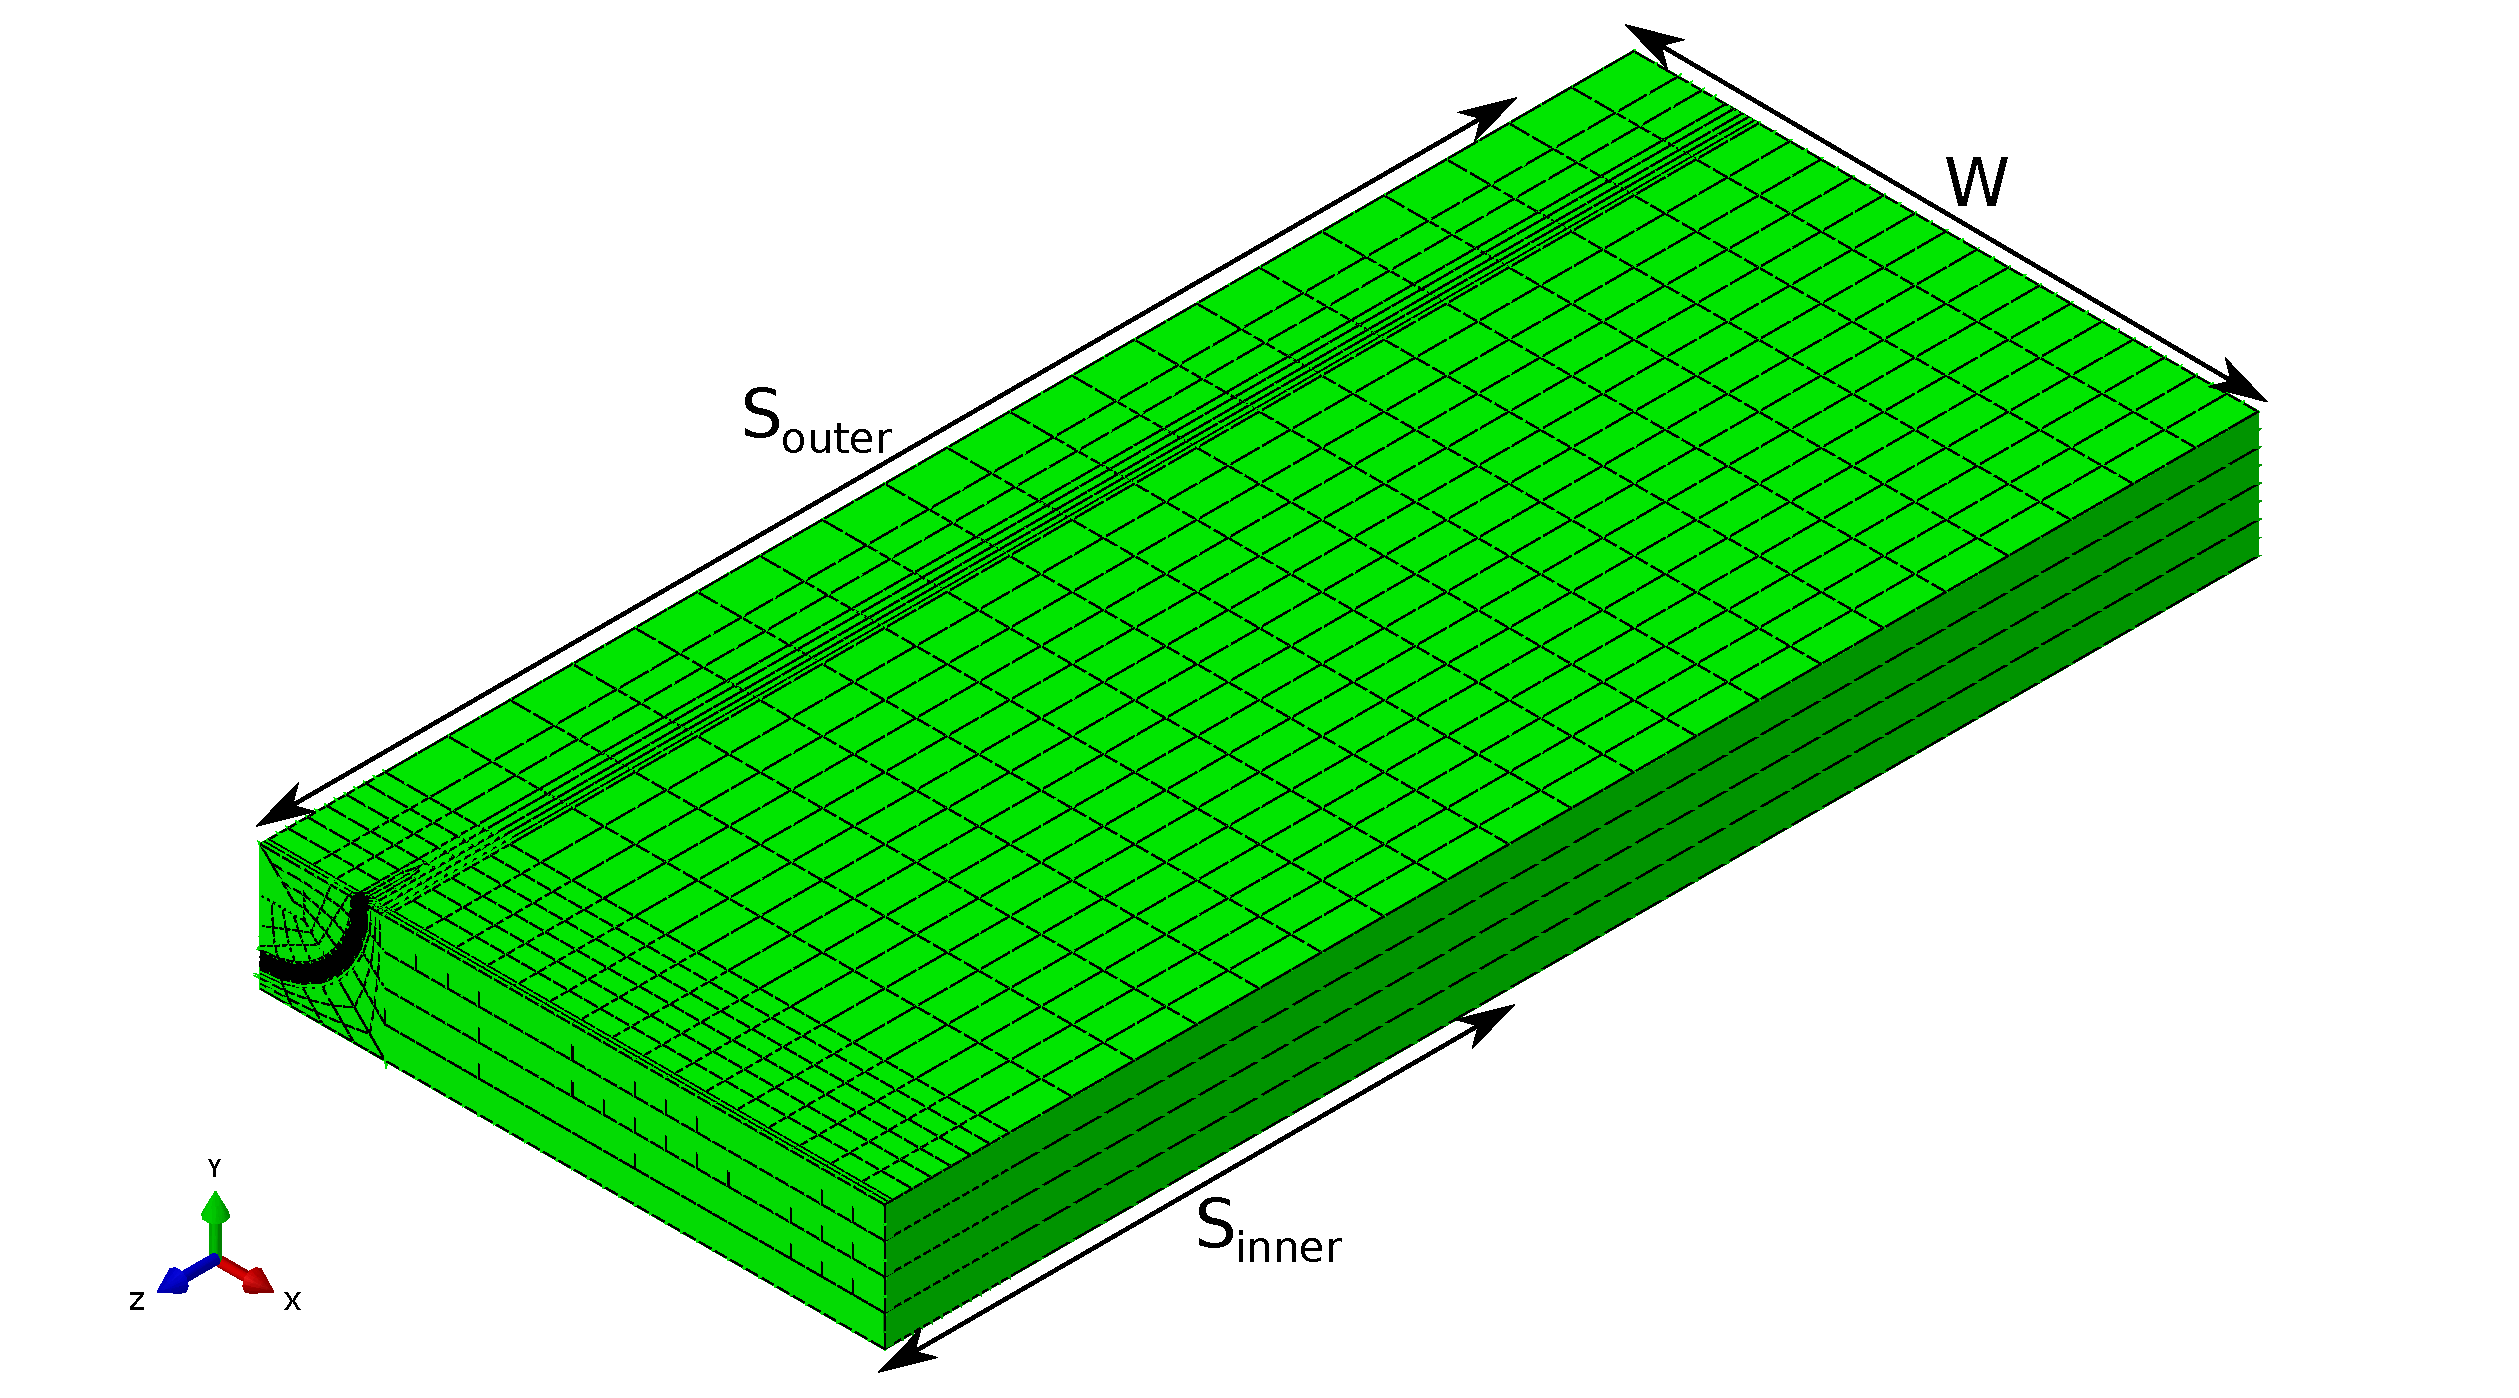
\includegraphics[width=\columnwidth]{mesh-iso-dimensioned}
\caption{\label{fig:mesh-iso-dimensioned}Model dimensions for plates in bending}
\end{figure}
Two example plates are shown in \Cref{fig:bend_ac02_at08_E0100_n03,fig:bend_ac10_at02_E0100_n03}, where each plate occupies extreme positions in terms of the crack geometry (and the plate width and length which are functions of crack width).
\begin{figure}[tbp]
\centering
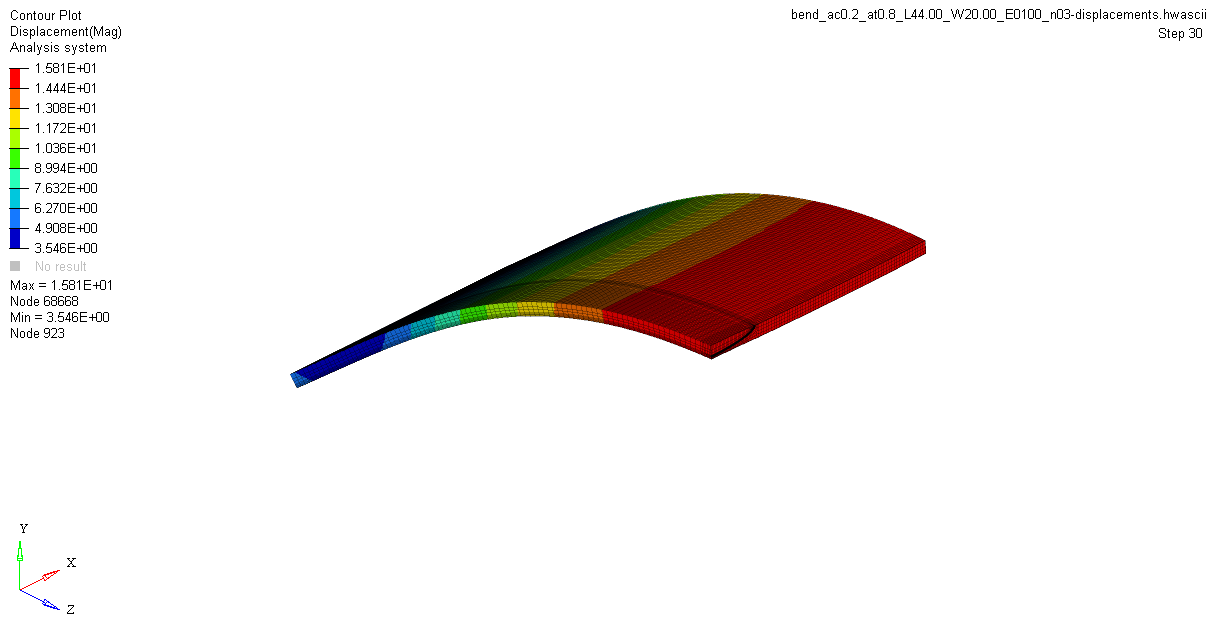
\includegraphics[width=\textwidth]{bend_ac02_at08_E0100_n03}
\caption{\label{fig:bend_ac02_at08_E0100_n03} Plate model, \(\frac{a}{c}=0.2\), \(\frac{a}{t}=0.8\)}
\end{figure}
\begin{figure}[tbp]
\centering
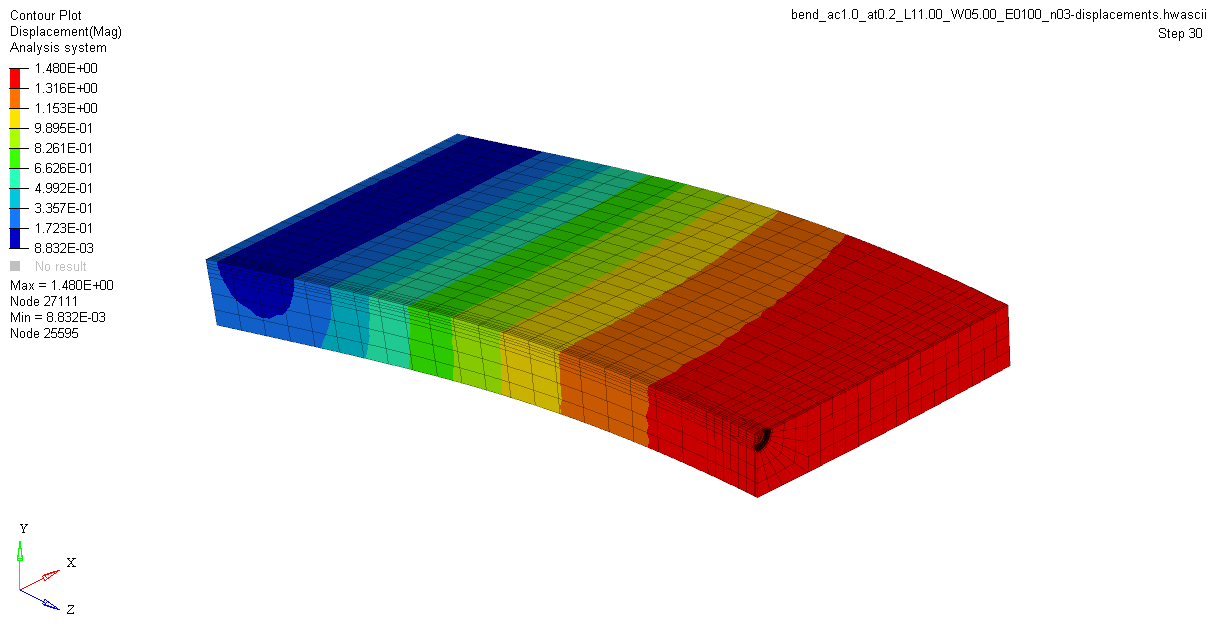
\includegraphics[width=\textwidth]{bend_ac10_at02_E0100_n03}
\caption{\label{fig:bend_ac10_at02_E0100_n03} Plate model, \(\frac{a}{c}=1.0\), \(\frac{a}{t}=0.2\)}
\end{figure}

After the geometry and mesh for a given cracked plate have been defined, the elastic modulus \(E\) and the plastic stress-strain curve must be defined.
Finally, each combination of plate geometry, mesh, and material properties must be written into separate WARP3D input files for analysis.
An algorithm for constructing these input files is given in \Cref{alg:plate-creator}, a Python version of the algorithm for a subset of the problem space is given in \Cref{lst:plate-creator,lst:bend-config}, and an overall flow chart of the program is given in \Cref{fig:plate-creator-flowchart}.
The \verb|numpy| numeric Python libraries \cite{numpy} are used throughout the plate creation process to simplify any array-based operations. 
\begin{algorithm}[tbp]
  \caption{Plate Creator}
  \label{alg:plate-creator}
  \begin{algorithmic}
    \Procedure{Plate Creator}{} \Comment{Create a series of WARP3D input files}
    \State Read lists of $\frac{a}{t}$, $\frac{a}{c}$, $\frac{E}{\sigma_{\text{ys}}}$, $n$ values from configuration
    \State \Comment{typically: $0.2 \leq \frac{a}{t} \leq 0.8$, $0.2 \leq \frac{a}{c} \leq 1.0$, $100 \leq \frac{E}{\sigma_\text{ys}} \leq 1000$, $3 \leq n \leq 20$}
    \State Read $t$, $\sigma_\text{ys}$, global .elt file from configuration
    \State \Comment{typically: $t=1$, $\sigma_\text{ys}=1$, and global .elt file = 'bend.elt'}
    \ForAll{($\frac{a}{t}$ values, $\frac{a}{c}$ values)}
      \State $(a, c, L, W, S_{\text{in}}, S_{\text{out}}) \gets \Call{Set Geometry}{\text{global .elt file}, \frac{a}{c}, \frac{a}{t}, t}$
      \State $\text{generic mesh} \gets \Call{Build Mesh}{\text{global .elt file}, a, c, t, L, W, S_{\text{in}}, S_{\text{out}}}$
      \State \Comment{creates an input file with an arbitrary material for every combination of $\frac{a}{c}$ and $\frac{a}{t}$}
      \ForAll{($\frac{E}{\sigma_\text{ys}}$ values, $n$ values)}
        \State $E \gets (\frac{E}{\sigma_\text{ys}})(\sigma_\text{ys})$
        \State $\text{WARP3D input} \gets \Call{Set Material}{\text{generic mesh}, E, \sigma_\text{ys}, n}$
        \State \Comment{creates an input file for every combination of $\frac{a}{c}$, $\frac{a}{t}$, $E$, and $n$}
      \EndFor
    \EndFor
    \EndProcedure
  \end{algorithmic}
\end{algorithm}
\begin{Spacing}{1}
\begin{lstlisting}[language=Python,caption={Python implementation of Plate Creator algorithm}, label=lst:plate-creator]
# plate_creator.py
import preprocess as pre
from bend_config import aspect_ratio_list, depth_ratio_list
from bend_config import plate_thickness, E_Sys_ratio_list
from bend_config import Sys, n_list
from bend_config import elt_global_template_filename

for depth_ratio in depth_ratio_list:
    for aspect_ratio in aspect_ratio_list:
        (a, c, W, t, L,
         S_inner, S_outer) = pre.calculate_geometry(
                     elt_global_template_filename,
                     depth_ratio, aspect_ratio,
                     plate_thickness)
        geom_filename = pre.build_mesh(
                elt_global_template_filename, a, c, L, W, t,
                S_inner, S_outer)
        print("Wrote generic mesh {0}".format(geom_filename))
        for n in n_list:
            for E_Sys_ratio in E_Sys_ratio_list:
                E = Sys*E_Sys_ratio
                model_filename = pre.change_material_properties(
                        inp_filename=geom_filename,
                        E=E, Sys=Sys, n=n)
                print("Wrote {0}".format(model_filename))
\end{lstlisting}
\end{Spacing}
\begin{Spacing}{1}
\begin{lstlisting}[language=Python,caption={Python implementation for subset of geometry and material configurations}, label=lst:bend-config]
# bend_config.py
aspect_ratio_list = [0.2, 0.4, ]
depth_ratio_list = [0.2, 0.4, 0.6, 0.8, ]
plate_thickness = 1.0
E_Sys_ratio_list = [100.0, 200.0, 300.0, 500.0, 700.0, 1000.0, ]
Sys = 1.0
n_list = [3, 4, 6, 10, 20, ]
elt_global_template_filename = 'bend.elt'
\end{lstlisting}
\end{Spacing}
\begin{figure}
\centering
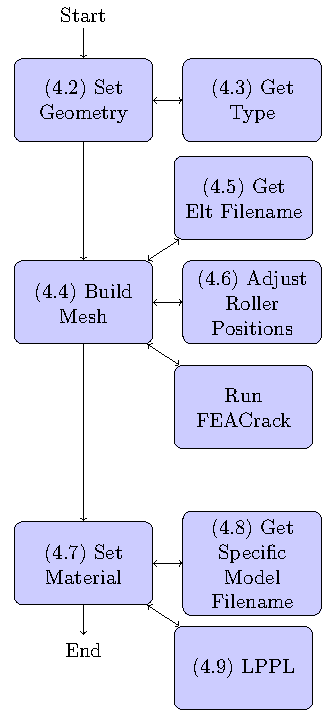
\includegraphics[width=0.5\columnwidth]{plate_creator_flowchart}
\caption{\label{fig:plate-creator-flowchart} Overall flowchart of bending model creation program}
\end{figure}


The remaining algorithms will be shown only as pseudocode in order to emphasize the structure of the algorithms instead of their specific implementation.
Readers interested in the Python implementation can download a copy of the Python source files from \url{https://github.com/mikerenfro/phd}.

\subsection{Defining Plate Model Geometry}

\Cref{alg:set_geometry} uses \Cref{alg:get_type} to determine if the model is in bending or tension, and calculates the necessary plate dimensions from given values for crack aspect ratio, crack depth ratio, and plate thickness.
\Cref{alg:get_type} looks through an FEACrack input file for specific commands in the file's notes field and commands.
If a traction in the \(y\) direction is defined in the notes field, and two rigid roller surfaces are found in the model commands, the model is assumed to represent a plate in bending.
Otherwise, the model is assumed to represent a plate in tension.
\Cref{alg:build_mesh} has four main tasks: to first use \Cref{alg:get_elt_filename} to define the name of a new FEACrack input file, to copy the generic FEACrack input file to the new name, to use \Cref{alg:adjust_roller_positions} to modify the roller locations for bending models, and finally running FEACrack with command arguments to create a WARP3D input file with the correct plate geometry and crack size.
\Cref{alg:get_elt_filename} takes the name of the generic FEACrack input file and a list of dimension values, and defines a new FEACrack input filename with the dimension values included.
\Cref{alg:adjust_roller_positions} searches an FEACrack input file for commands representing the position of rollers, and changes their \(z\) dimensions to match \Sinner and \Souter.
\begin{algorithm}[tbp]
  \caption{Set Geometry}
  \label{alg:set_geometry}
  \begin{algorithmic}
    \Procedure{Set Geometry}{$\text{global .elt file}, \frac{a}{c}, \frac{a}{t}, t$} \Comment{Calculate plate dimensions}
    \State $a \gets (\frac{a}{t})t$
    \State $c \gets a (\frac{a}{c})^{-1}$
    \If{$c > t$}
      \State $W \gets 5c$
    \Else
      \State $W \gets 5t$
    \EndIf
    \State $\text{model type} \gets \Call{Get Type}{\text{global .elt file}}$
    \If{model type = 'bending'}
      \State $\Sinner \gets W$
      \State $\Souter \gets 2W$
      \If{$2 W > 1.1 \Souter$}
        \State $L \gets 2 W$
      \Else
        \State $L \gets 1.1 \Souter$
      \EndIf
    \Else
      \State $\Sinner \gets \text{Null}$
      \State $\Souter \gets \text{Null}$
      \State $L \gets 2 W$
    \EndIf
    \State \textbf{return} $(a, c, W, L, \Sinner, \Souter)$
    \EndProcedure
  \end{algorithmic}
\end{algorithm}

\begin{algorithm}[tbp]
  \caption{Get Type}
  \label{alg:get_type}
  \begin{algorithmic}
    \Procedure{Get Type}{global .elt file}
      \State \Comment{determine if a .elt file is for a bending or a tension model}
      \If{'"*use bottom load pin plate ty ' found in 'Notes:' field}
        \If{'RigidSurfaceData\_Radius' found twice}
          \If{'RigidSurfaceData\_PinLocation' found twice}
            \State model type $\gets$ 'bending'
          \Else
            \State model type $\gets$ 'invalid'
          \EndIf
        \EndIf
      \Else
        \State model type $\gets$ 'tension'
      \EndIf
      \State \textbf{return} model type
    \EndProcedure
  \end{algorithmic}
\end{algorithm}

\begin{algorithm}[tbp]
  \caption{Build Mesh}
  \label{alg:build_mesh}
  \begin{algorithmic}
    \Procedure{Build Mesh}{{global .elt file}, $a$, $c$, $t$, $L$, $W$, $\Sinner$, $\Souter$}
      \State \Comment{use FEACrack create a WARP3D input file with an arbitrary material}
      \State {model .elt file} $\gets$ \Call{Get Elt Filename}{{global .elt file}, $a$, $c$, $L$, $W$, $t$} 
      \State \Comment{'bend\_ac$(\frac{a}{c})$\_at$(\frac{a}{t})$\_L$(L)$\_W$(W)$.elt'}
      \State Copy {global .elt file} to {model .elt file}
      \If{$\Sinner \neq \text{Null} \AND \Souter \neq \text{Null}$}
        \State \Call{Adjust Roller Positions}{model .elt file, $\Sinner$, $\Souter$}
      \EndIf
      \State Run FEACrack program on model .elt file, using $a$, $2c$, $t$, $L$, and $W$
      \State \textbf{return} \text{generic mesh file} \Comment{'bend\_ac$(\frac{a}{c})$\_at$(\frac{a}{t})$\_L$(L)$\_W$(W)$\_wrp.inp'}
    \EndProcedure
  \end{algorithmic}
\end{algorithm}

\begin{algorithm}[tbp]
  \caption{Get Elt Filename}
  \label{alg:get_elt_filename}
  \begin{algorithmic}
    \Procedure{Get Elt Filename}{global .elt file, $a$, $c$, $L$, $W$, $t$}
      \State \Comment{determine the name of a .elt file for a given geometry}
      \State prefix $\gets$ global .elt file basename \Comment{'bend'}
      \State middle $\gets$ '\_ac$(\frac{a}{c})$\_at$(\frac{a}{t})$\_L$(L)$\_W$(W)$'
      \State suffix $\gets$ '.elt'
      \State \textbf{return} prefix + middle + suffix \Comment{'bend\_ac$(\frac{a}{c})$\_at$(\frac{a}{t})$\_L$(L)$\_W$(W)$.elt'}
    \EndProcedure
  \end{algorithmic}
\end{algorithm}

\begin{algorithm}[tbp]
  \caption{Adjust Roller Positions}
  \label{alg:adjust_roller_positions}
  \begin{algorithmic}
    \Procedure{Adjust Roller Positions}{model .elt file, $\Sinner$, $\Souter$}
    \State \Comment{move roller positions in .elt file to $\Sinner$ and $\Souter$}
    \If{first 'RigidSurfaceData\_PinLocation' found in model .elt file}
      \State Change $z$ value of location to $\Sinner$
    \EndIf
    \If{second 'RigidSurfaceData\_PinLocation' found in model .elt file}
      \State Change $z$ value of location to $\Souter$
    \EndIf
    \EndProcedure
  \end{algorithmic}
\end{algorithm}

\subsection{Defining Material Properties}

\Cref{alg:set_material} calls \Cref{alg:get_specific_model_filename} to determine the name of a WARP3D input file for a specific material, copies the WARP3D input file for the current geometry to the new name, and examines the new WARP3D input file for lines representing the plastic behavior of the material. Those lines are replaced with the results of \Cref{alg:lppl} for a given elastic modulus, yield strength, and hardening exponent.
\Cref{alg:get_specific_model_filename} takes the name of the WARP3D file for the current geometry and defines a new WARP3D input filename with the elastic modulus and hardening exponent values included.
\Cref{alg:lppl} defines a set of plastic strain values that are finely spaced near the onset of yield, and increasingly coarse as plastic strain increases, and uses a power law relationship to define the corresponding set of true stress values. This ensures a smooth transition from linear behavior without using an excessive total number of points on the curve.

\begin{algorithm}[tbp]
  \caption{Set Material}
  \label{alg:set_material}
  \begin{algorithmic}
    \Procedure{Set Material}{generic .inp file, $E$, $\sigma_\text{ys}$, $n$}
    \State \Comment{modify arbitrary material parameters in input file to specified values}
    \State specific .inp file $\gets$ \Call{Get Specific Model Filename}{generic .inp file, $E$, $\sigma_\text{ys}$, $n$}
    \State \Comment{'bend\_ac$(\frac{a}{c})$\_at$(\frac{a}{t})$\_L$(L)$\_W$(W)$\_E$(E)$\_n$(n)$\_wrp.inp'}
    \State Copy generic .inp file to specific .inp file
    \If{'stress-strain curve      1' found in specific .inp file}
      \State change stress-strain curve data to \Call{LPPL}{$E$, $\sigma_\text{ys}$, $n$}
    \EndIf
    \State change $E$ value in specific .inp file
    \State \textbf{return} specific .inp file \Comment{'bend\_ac$(\frac{a}{c})$\_at$(\frac{a}{t})$\_L$(L)$\_W$(W)$\_E$(E)$\_n$(n)$\_wrp.inp'}

    \EndProcedure
  \end{algorithmic}
\end{algorithm}

\begin{algorithm}[tbp]
  \caption{Get Specific Model Filename}
  \label{alg:get_specific_model_filename}
  \begin{algorithmic}
    \Procedure{Get Specific Model Filename}{.inp filename, $E$, $\sigma_\text{ys}$, $n$}
      \State \Comment{determine the name of a specific .inp file for a given geometry and material parameters}
      \State prefix $\gets$ .inp file basename \Comment{'bend\_ac$(\frac{a}{c})$\_at$(\frac{a}{t})$\_L$(L)$\_W$(W)$\_wrp'}
      \State prefix $\gets$ prefix without last 4 characters
      \State \Comment{'bend\_ac$(\frac{a}{c})$\_at$(\frac{a}{t})$\_L$(L)$\_W$(W)$'}
      \State middle $\gets$ '\_E$(E)$\_n$(n)$'
      \State suffix $\gets$ '\_wrp.inp'
      \State \textbf{return} prefix + middle + suffix
      \State \Comment{'bend\_ac$(\frac{a}{c})$\_at$(\frac{a}{t})$\_L$(L)$\_W$(W)$\_E$(E)$\_n$(n)$\_wrp.inp'}
    \EndProcedure
  \end{algorithmic}
\end{algorithm}

\begin{algorithm}[tbp]
  \caption{LPPL}
  \label{alg:lppl}
  \begin{algorithmic}
    \Procedure{LPPL}{$E$, $\sigma_\text{ys}$, $n$} \Comment{calculate the plastic stress-strain curve for a power law material}
    \State $\epsilon_{\text{pl1}} \gets (0.001, 0.002, \cdots , 0.008)$
    \State $\epsilon_{\text{pl2}} \gets (0.013, 0.018, 0.023, 0.028)$
    \State $\epsilon_{\text{pl3}} \gets (0.038, 0.048, \cdots , 0.108)$
    \State $\epsilon_{\text{ys}} \gets \frac{\sigma_\text{ys}}{E}$
    \State $\epsilon \gets \epsilon_{\text{ys}} + (\epsilon_{\text{pl1}}, \epsilon_{\text{pl2}}, \epsilon_{\text{pl3}})$
    \State $\sigma \gets \sigma_\text{ys}  (\frac{\epsilon}{\epsilon_{\text{ys}}})^{\frac{1}{n}}$
    \State \textbf{return} $\epsilon$, $\sigma$
    \EndProcedure
  \end{algorithmic}
\end{algorithm}

\section{Solving Plate Models, Optimizing Boundary Conditions}
\label{sec:solve}

Now that the plate geometry, material properties, and boundary conditions are defined for a set of models, a procedure for solving for reaction forces, \J values, and CMOD values must be developed.
The boundary conditions applied to the model must be large enough to induce substantial amounts of plastic deformation, but not so large as to cause the model to exceed its material limits or become numerically unstable.
In \cite{allenwells2014}, the models were reported to have been deformed enough to cause the deformation level\nomenclature[1M]{\(M\)}{dimensionless deformation parameter for plates in bending}
\begin{align}
M &= \frac{r_{\phi} \Sys}{\J}
\end{align}
to drop below 20 or 25, but upon examining the TASC database, approximately half the models had minimum \(M\) values over 25, and about 10\% of the models had \(M\) values over 50, as seen in \Cref{fig:min-M-hist}.
Regardless of the exact deformation required, all models in the TASC database must contain enough data to perform accurate linear extrapolations from the \(\sigma\)-CMOD and \J-CMOD curves, similar to the curves shown in \Cref{fig:J-CMOD-extrapolation}.

\begin{figure}[tbp]
\centering
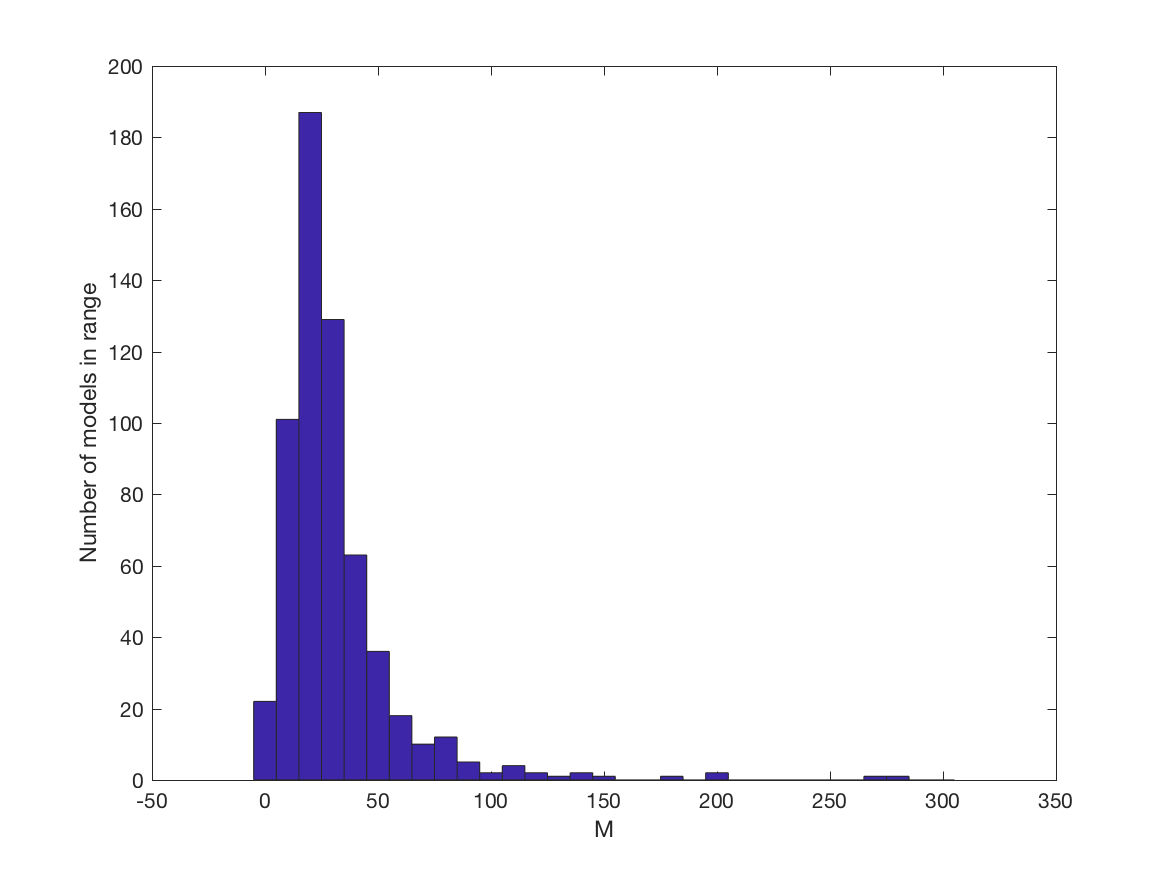
\includegraphics[width=0.7\columnwidth]{min_M_hist}
\caption{\label{fig:min-M-hist} Histogram of \(M\) results from TASC tension model database}
\end{figure}

\begin{figure}[tbp]
\centering
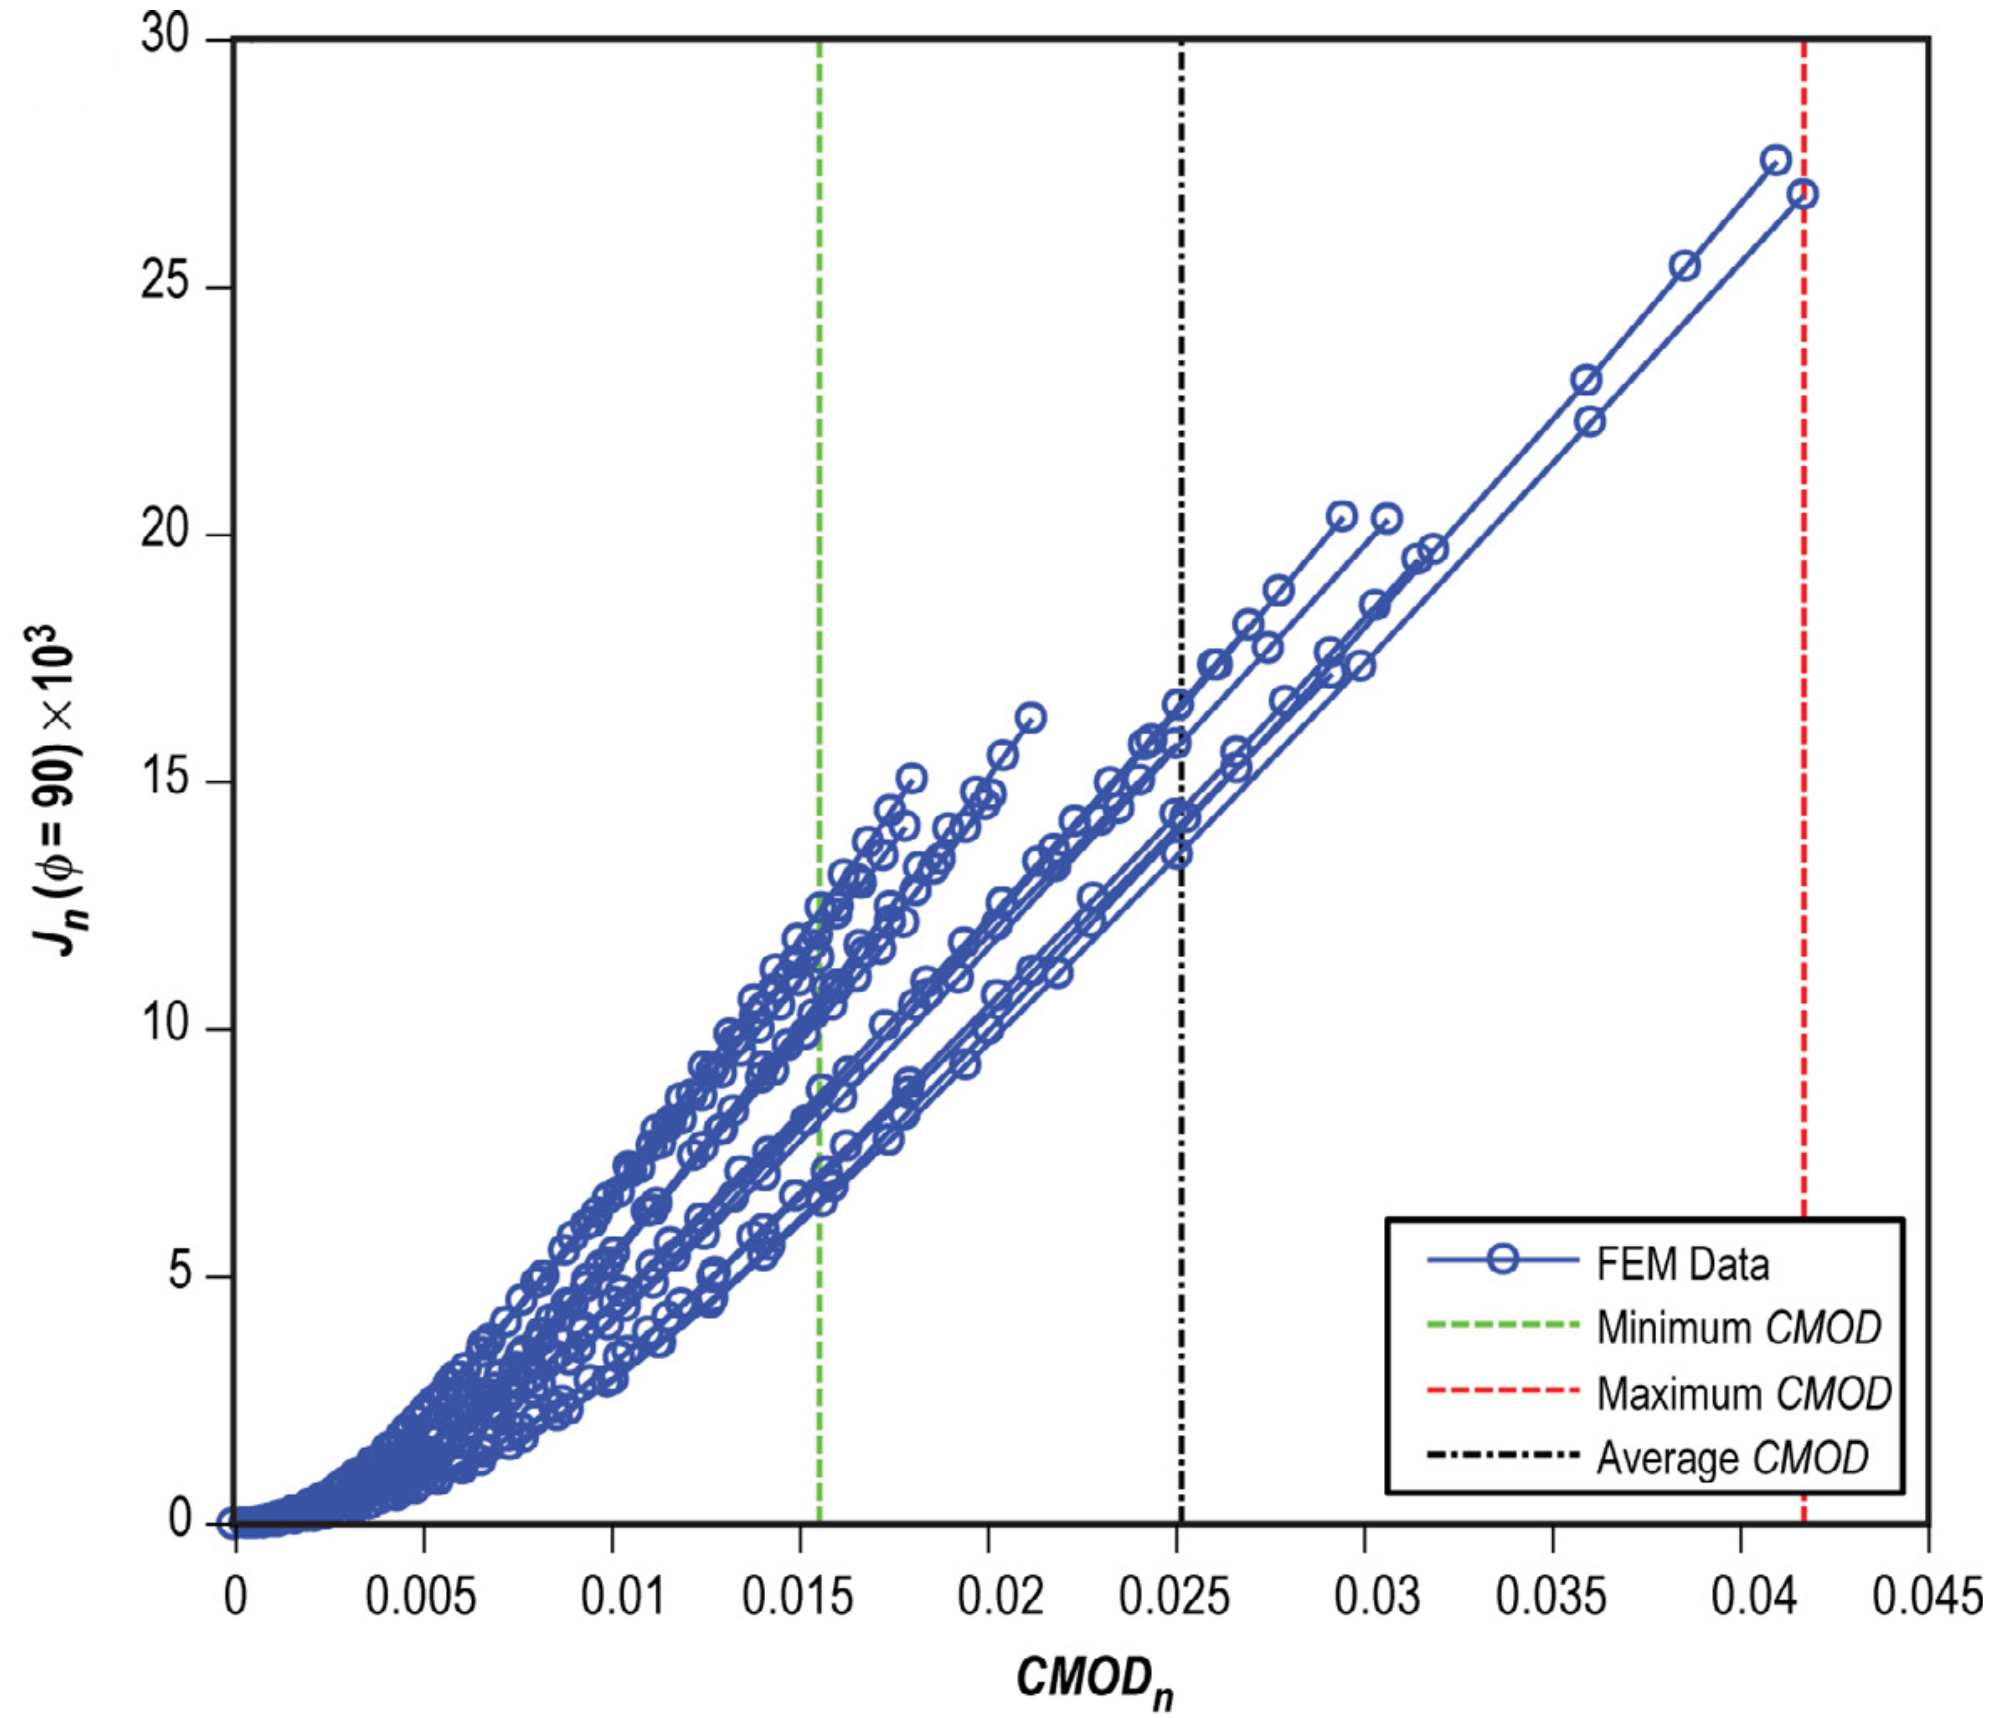
\includegraphics[width=0.7\columnwidth]{J-CMOD-extrapolation}
\caption[\J-CMOD graph used for extrapolation]{\label{fig:J-CMOD-extrapolation} \J-CMOD graph used for extrapolation \cite{allenwells2014}}
\end{figure}

\J{}-CMOD curves like the ones in \Cref{fig:J-CMOD-extrapolation,fig:J-phi-ac_02_at_02_E0100_n03,fig:J-phi-ac_10_at_08_E0500_n06} all show \J values that increase slowly in the linear elastic regime compared to the highly-plastic regime, but have widely varying \J and CMOD ranges.
Some cracks in bending will show lower \J values at the free surface than deep inside the crack, as shown in \Cref{fig:J-phi-ac_02_at_02_E0100_n03}, while others will show higher \J values at the free surface than deep inside the crack, as shown in \Cref{fig:J-phi-ac_10_at_08_E0500_n06}.
\begin{figure}[tbp]
\centering
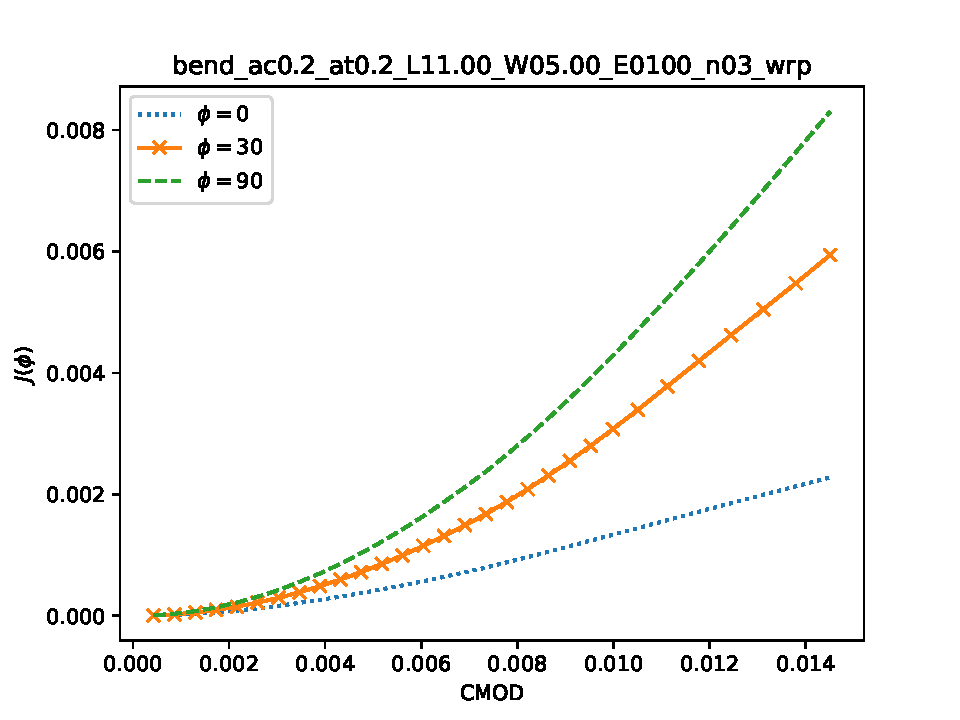
\includegraphics[width=0.8\textwidth]{J_CMOD_bend_ac02_at02_L1100_W0500_E0100_n03_wrp}
\caption{\J-CMOD relationship at \(\phi=\) \SIlist{0;30;90}{\SIUnitSymbolDegree}: \(\frac{a}{c}=0.2\), \(\frac{a}{t}=0.2\), \(E=100\), \(n=3\) \label{fig:J-phi-ac_02_at_02_E0100_n03}}
\end{figure}
\begin{figure}[tbp]
\centering
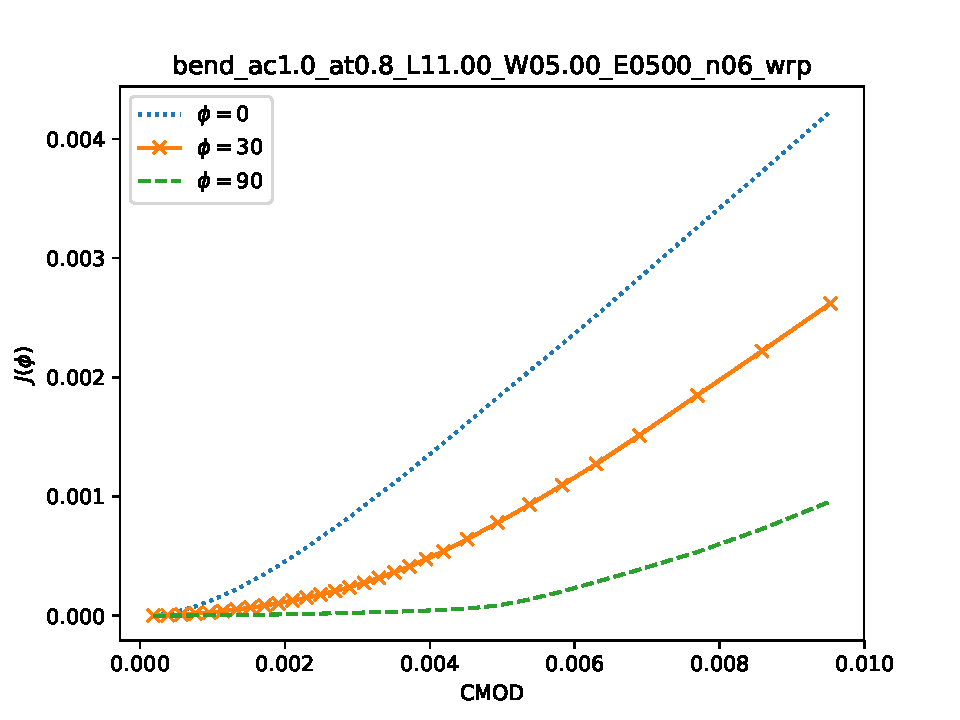
\includegraphics[width=0.8\textwidth]{J_CMOD_bend_ac10_at08_L1100_W0500_E0500_n06_wrp}
\caption{\J-CMOD relationship at \(\phi=\) \SIlist{0;30;90}{\SIUnitSymbolDegree}: \(\frac{a}{c}=1.0\), \(\frac{a}{t}=0.6\), \(E=500\), \(n=6\) \label{fig:J-phi-ac_10_at_08_E0500_n06}}
\end{figure}
Since the goal with a bending model is to use enough deformation to make accurate linear extrapolations from the results, the criteria analogous to the \(M\) criteria from \cite{allenwells2014} is defined as
\begin{enumerate} \label{list:criteria}
\item the slope of a linear fit to the last 20\% of the \J-CMOD curve should be at least 20 times larger than the slope of the initial linear region of the \J-CMOD curve, and
\item the slope of the last 20\% of the \J-CMOD curve should be within 10\% of the slope of the previous 20\% of the \J-CMOD curve.
\end{enumerate}
The first criteria ensures that the model has deformed well beyond the linear elastic regime, and the second ensures that linear extrapolations will be relatively insensitive to additional deformation.
Using ratios of \J and CMOD values in both criteria removes variability due to material properties and crack geometry.
As \J at a given CMOD is a function of angle \(\phi\) from the free surface, the \J values for \(\phi=30{\SIUnitSymbolDegree}\) are used to avoid effects of both the stress-free surface at \SI{0}{\SIUnitSymbolDegree} and constraint effects at \SI{90}{\SIUnitSymbolDegree}.

An algorithm for solving a set of models created by \Cref{alg:plate-creator} is shown in \Cref{alg:plate-runner}, with an overall flow chart shown in \Cref{fig:plate_runner_flowchart}.
For each combination of \(\frac{a}{c}\), \(\frac{a}{t}\), \(\frac{E}{\sigma_{\text{ys}}}\), and \(n\), it uses \Cref{alg:set_geometry} to calculate the cracked geometry.
It uses \Cref{alg:get_elt_filename,alg:get_generic_model_filename,alg:get_specific_model_filename} to identify relevant input files, and uses \Cref{alg:optimize_bc} to automate the process of modifying boundary conditions and solving the finite element models until the plates have been sufficiently deformed to satisfy the the list of criteria on \cpageref{list:criteria}.
The Python implementation of these algorithms makes use of the \verb|numpy| \cite{numpy}, \verb|scipy| \cite{scipy}, and  \verb|pandas| \cite{mckinney-proc-scipy-2010} libraries.
\verb|numpy| is used as a general-purpose numerical library for Python, \verb|scipy| is used for both linear regressions and optimizations, while \verb|pandas| is used for reading and filtering structured output files.
\begin{figure}
\centering
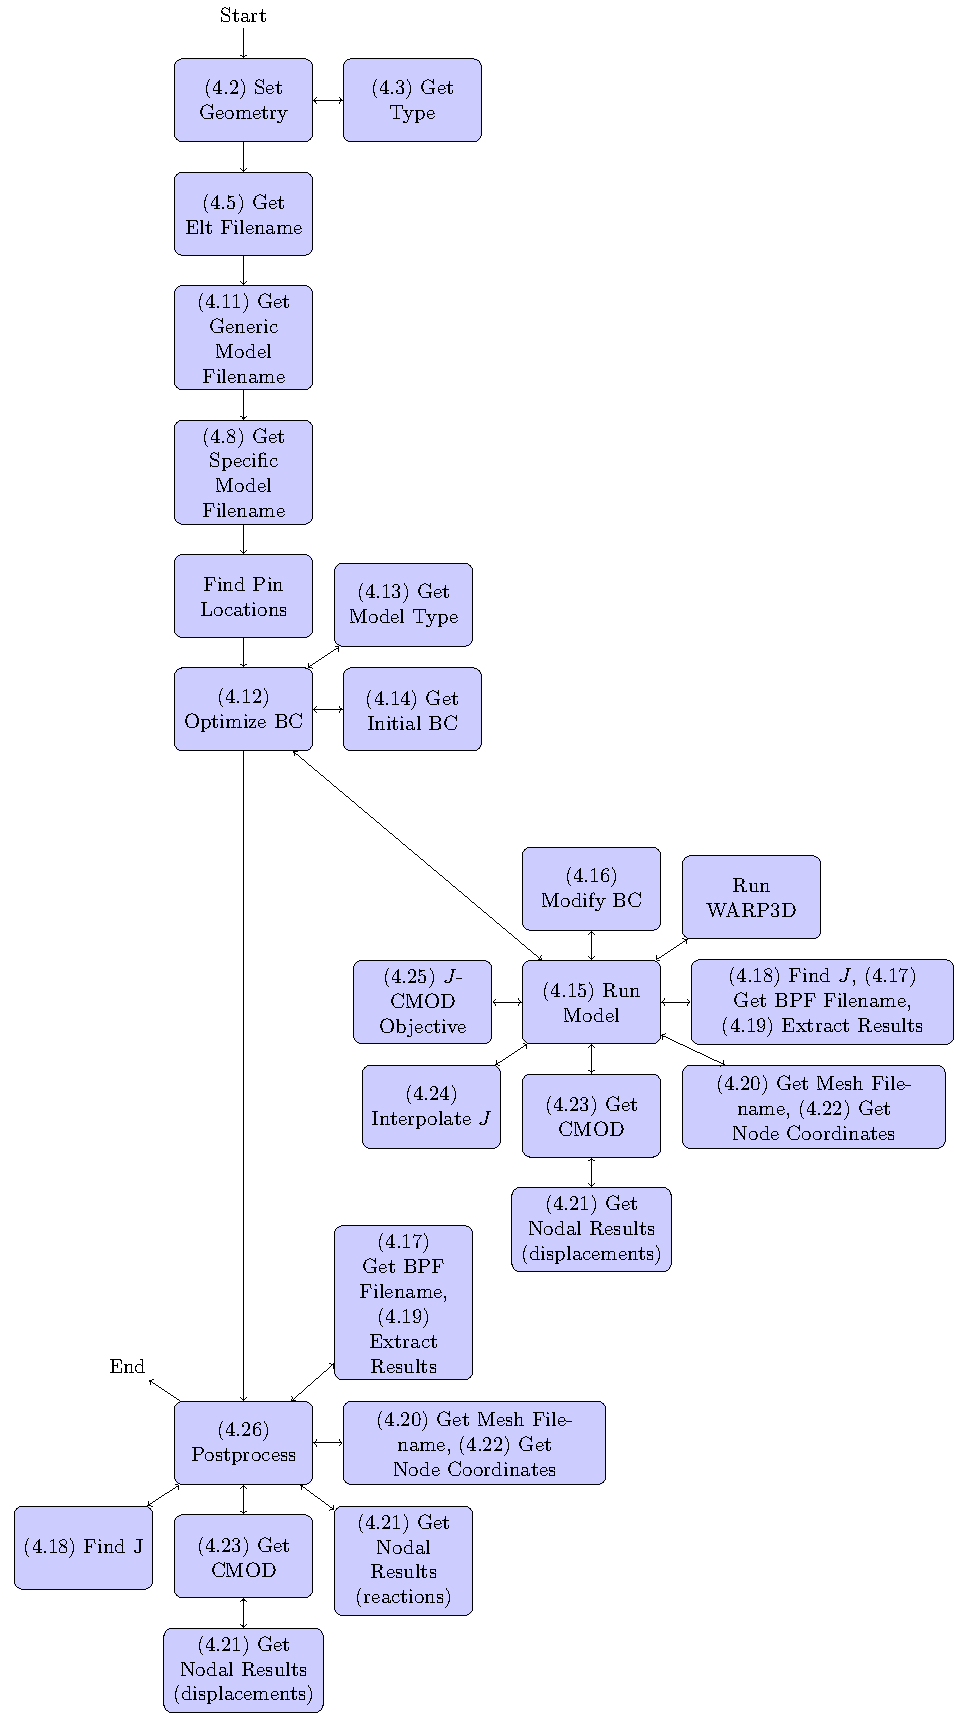
\includegraphics[width=0.75\columnwidth]{plate_runner_flowchart}
\caption{\label{fig:plate_runner_flowchart} Overall flowchart of bending model solution program}
\end{figure}


Looking more closely at the process for finding boundary conditions as shown in \Cref{alg:optimize_bc}, the following details must be considered.
All the materials examined have highly non-linear stress-strain (and load-displacement) behavior, where small changes in applied stresses or loads may cause large changes in strains or displacements.
Similarly, large changes in strain or displacement may only cause small changes in stress or reaction loads.
Displacement boundary conditions were used in \cite{allenwells2014}, which mimics common closed-loop control methods used in mechanical properties testing.
These boundary conditions were constant values applied on the face parallel to the crack front.
However, reaching a sufficient level of plastic deformation around the crack front may require much more displacement than required to reach yield, as shown in \Cref{fig:secant-1}.
\begin{figure}[tbp]
\centering
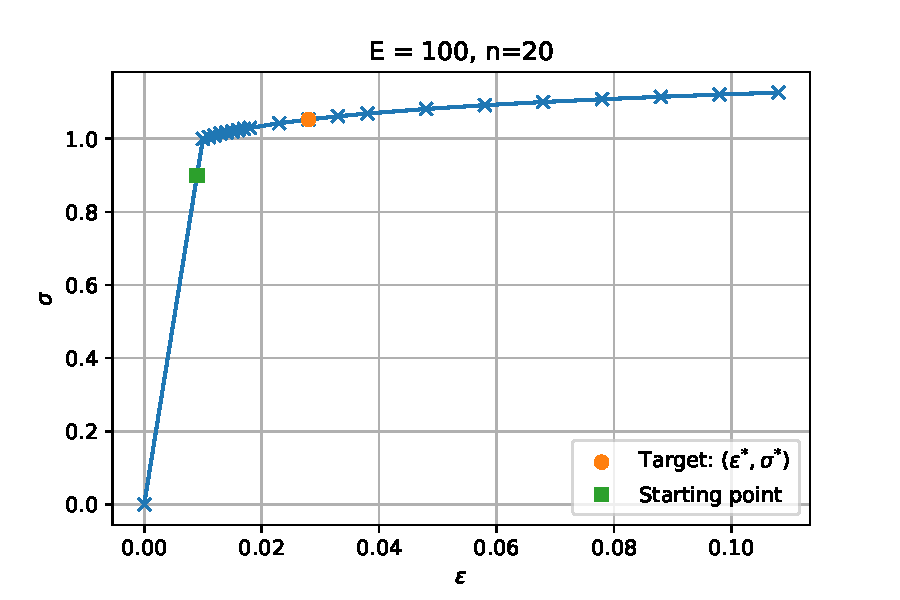
\includegraphics[width=0.8\columnwidth]{secant-1}
\caption{\label{fig:secant-1}Example stress-strain curve using linear plus power law (LPPL) formulation}
\end{figure}
Applying an incremental search to discover how much displacement is required to reach that level of plastic deformation would prove to be slow to converge (where small displacement steps cause even smaller changes in stress state for most of the search space) or inaccurate (where large displacement steps risk running outside the material's defined stress-strain data).
Considering a transformed stress-strain curve as shown in \Cref{fig:secant-2} where the starting point on the stress-strain curve is shown by the green square, the secant method should converge quickly to the target point shown by the orange circle.
\begin{figure}[tbp]
\centering
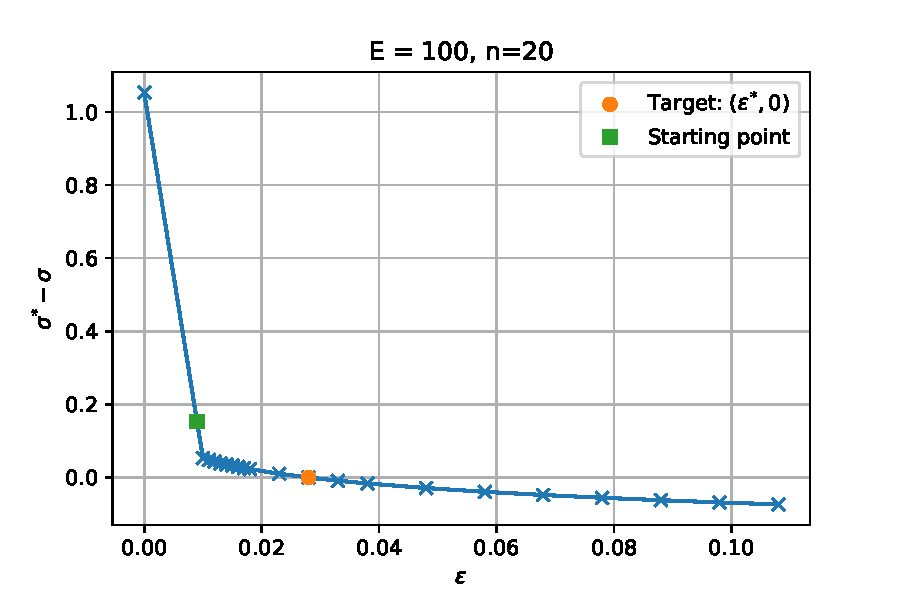
\includegraphics[width=0.8\columnwidth]{secant-2}
\caption{\label{fig:secant-2}LPPL stress-strain curve, transformed to find required strain level}
\end{figure}

The bending models require additional considerations to match experimental conditions, especially for larger plates.
A typical four-point bend test applies external forces with a set of inner cylindrical rollers, and the plate is supported by an outer set of cylindrical rollers, as shown in \Cref{fig:astm-e2899-4point-bend}.
Modeling the internal rollers as constant transverse displacement conditions along a plane parallel to the crack face will grow increasingly inaccurate as that plane rotates relative to the crack face.
Applying transverse tractions on all element faces coincident with the location of the inner roller solves this issue.
Because traction has units of force per unit area, the same traction value can be applied to each element, regardless of the element size.
\begin{figure}[tbp]
\centering
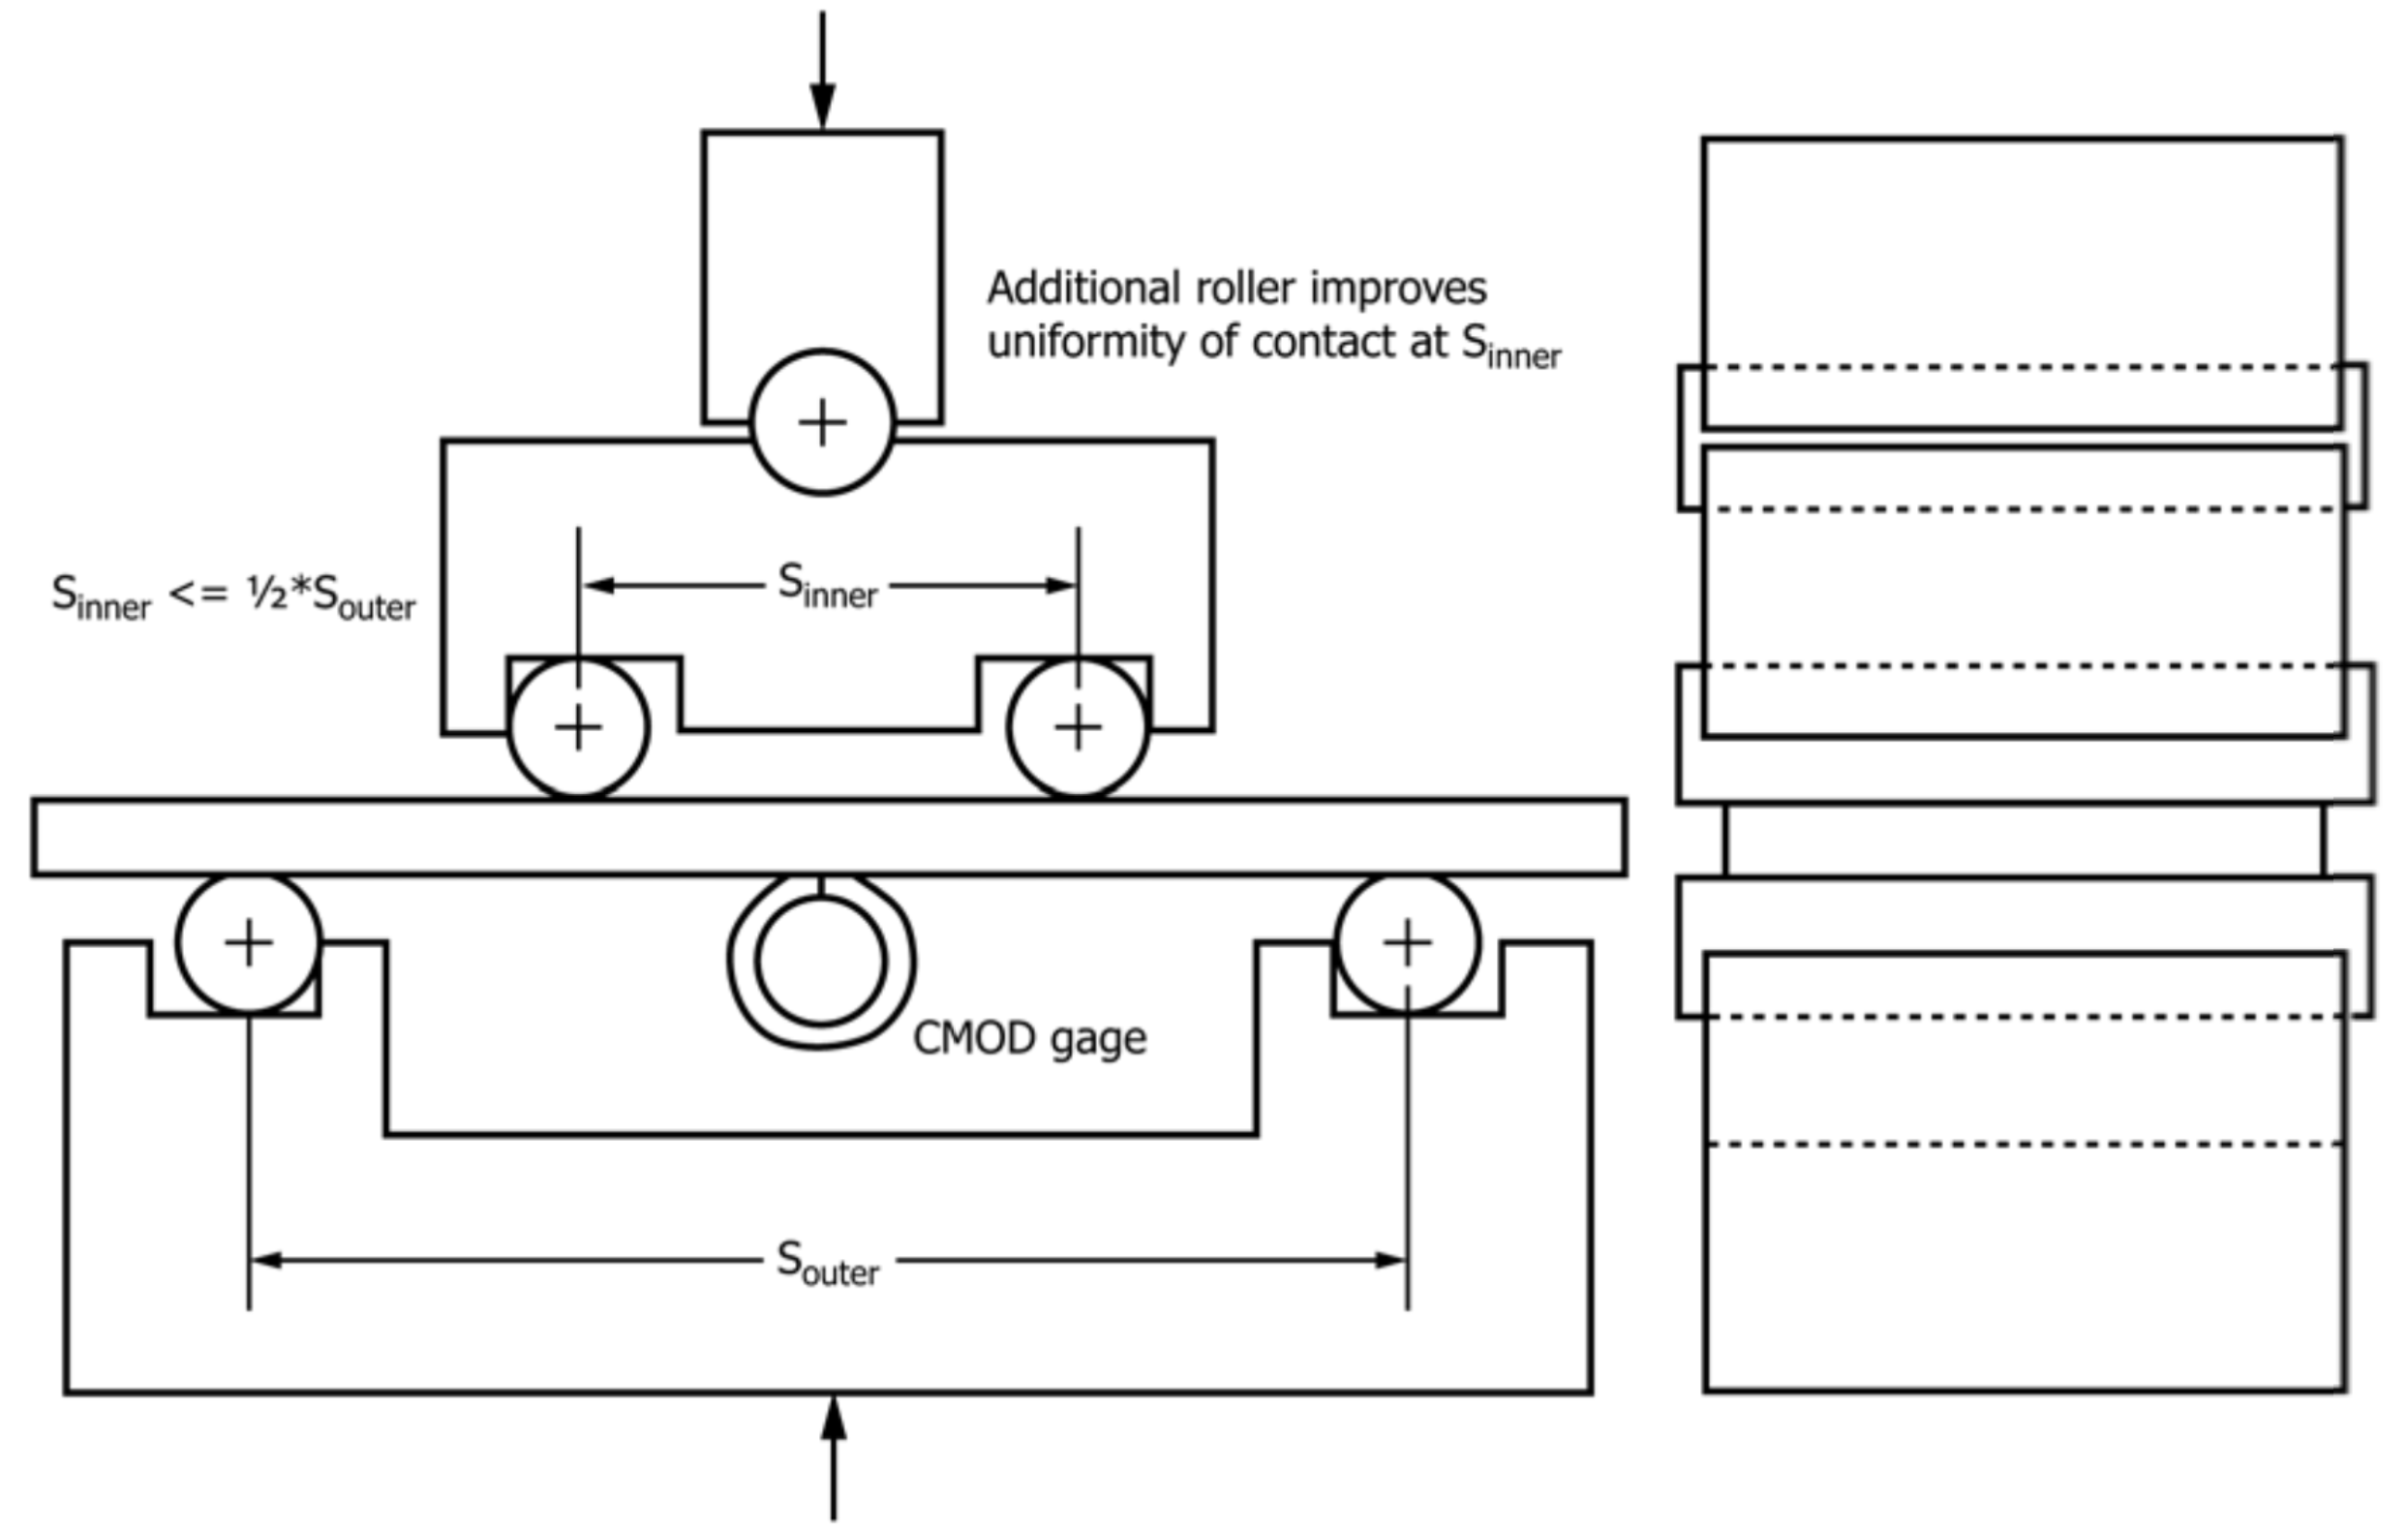
\includegraphics[width=0.8\columnwidth]{astm-e2899-4point-bend}
\caption[Four-point bend test configuration]{\label{fig:astm-e2899-4point-bend} Four-point bend test configuration \cite{astme2899}}
\end{figure}

However, moving from a strain- or displacement-controlled method to a stress- or force-controlled method complicates the root-finding methods used in the tension cases.
As the independent variable is now stress, and the dependent variable is now strain, this transforms the stress-strain curve to the form shown in \Cref{fig:secant-3,fig:secant-4}.
\begin{figure}[tbp]
\centering
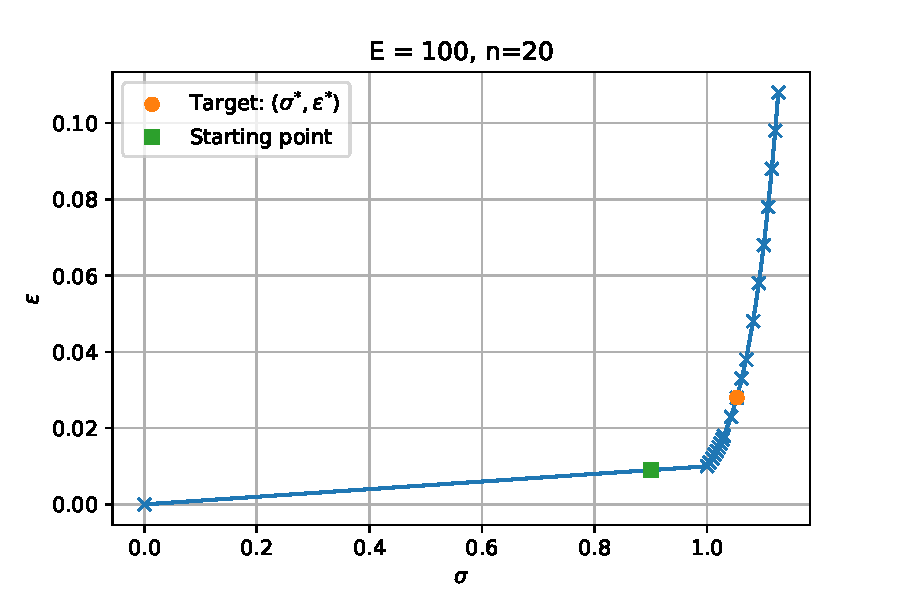
\includegraphics[width=0.8\columnwidth]{secant-3}
\caption{\label{fig:secant-3}Example stress-strain curve using linear plus power law (LPPL) formulation, transformed to stress-controlled}
\end{figure}
\begin{figure}[tbp]
\centering
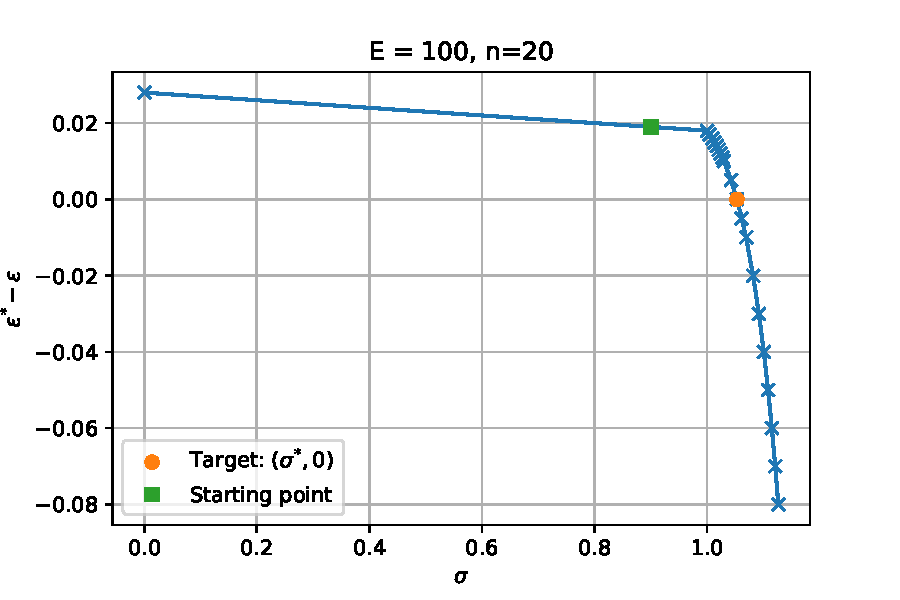
\includegraphics[width=0.8\columnwidth]{secant-4}
\caption{\label{fig:secant-4}Example stress-strain curve using linear plus power law (LPPL) formulation, transformed to find required stress level}
\end{figure}
The curve is now much less suitable for solution using the secant method: the neighborhood of starting point has a very shallow slope that will cause the next stress value to be much higher, either causing slow convergence in the case of an LPPL function with a semi-infinite domain, or simply exceeding the range of the stress-strain curve in the case of a finite set of stress-strain points.
However, using a simple incremental search method with step sizes equal to 10\% of the initial stress only takes a few steps to reach the neighborhood of the target stress value.
Other root-finding methods could be used to find the required stress value, such as bisection, false position, or Brent's method \cite{numericalrecipes1986}.
However, each of these methods requires the determination of a finite interval \([\sigma_a, \sigma_b]\) that surround the required stress value.
Though it is possible to set that interval to the domain of a finite set of stress-strain data points, this is impossible for an LPPL function with a semi-infinite domain.
Additionally, the open-ended nature of the slope ratio criteria on \cpageref{list:criteria} means that all stress values exceeding a minimum target value will meet that criteria.
Finally, having a finite number of load steps in the finite element model and the need to accurately model the transition to elastic-plastic behavior means that lower stress values meeting the criteria on \cpageref{list:criteria} are preferred.
All three of these factors lead to a conclusion that any root-finding method that requires no bracketing and whose proposed root values monotonically increase will find appropriate stress values that will allow accurate extrapolation without sacrificing detail in the transition to elastic-plastic behavior.
\begin{algorithm}[tbp]
  \caption{Plate Runner}
  \label{alg:plate-runner}
  \begin{algorithmic}
    \Procedure{Plate Runner}{} \Comment{Solve a series of WARP3D input files}
    \State Read lists of $\frac{a}{t}$, $\frac{a}{c}$, $\frac{E}{\sigma_{\text{ys}}}$, $n$ values from configuration
    \State \Comment{typically: $0.2 \leq \frac{a}{t} \leq 0.8$, $0.2 \leq \frac{a}{c} \leq 1.0$, $100 \leq \frac{E}{\sigma_\text{ys}} \leq 1000$, $3 \leq n \leq 20$}
    \State Read $t$, $\sigma_\text{ys}$, global .elt file from configuration
    \State \Comment{typically: $t=1$, $\sigma_\text{ys}=1$, and global .elt file = 'bend.elt'}
    \ForAll{($\frac{a}{t}$ values, $\frac{a}{c}$ values)}
      \State $(a, c, L, W, S_{\text{in}}, S_{\text{out}}) \gets \Call{Set Geometry}{\text{global .elt file}, \frac{a}{c}, \frac{a}{t}, t}$
      \ForAll{($\frac{E}{\sigma_\text{ys}}$ values, $n$ values)}
        \State $E \gets (\frac{E}{\sigma_\text{ys}})(\sigma_\text{ys})$
        \State {model .elt file} $\gets$ \Call{Get Elt Filename}{{global .elt file}, $a$, $c$, $L$, $W$, $t$} 
        \State \Comment{'bend\_ac$(\frac{a}{c})$\_at$(\frac{a}{t})$\_L$(L)$\_W$(W)$.elt'}
        \State {generic .inp file} $\gets$ \Call{Get Generic Model Filename}{{model .elt file}}
        \State \Comment{'bend\_ac$(\frac{a}{c})$\_at$(\frac{a}{t})$\_L$(L)$\_W$(W)$\_wrp.inp'}
        \State {specific .inp file} $\gets$ \Call{Get Specific Model Filename}{{generic .inp file}, $E$, $\sigma_\text{ys}$, $n$}
        \State \Comment{'bend\_ac$(\frac{a}{c})$\_at$(\frac{a}{t})$\_L$(L)$\_W$(W)$\_E$(E)$\_n$(n)$\_wrp.inp'}
        \If{\Call{Get Model Type}{specific .inp file} = 'bending'}
          \State ($z_{\text{in}}$, $z_{\text{out}}$) = \Call{Find Pin Locations}{specific .inp file}
        \EndIf
        \State \Call{Optimize BC}{specific .inp file, $a$, $c$, $L$, $W$, $t$, $z_{\text{in}}$, $z_{\text{out}}$, $E$, $n$}
        \State \Call{Postprocess}{specific .inp file}
      \EndFor
    \EndFor
    \EndProcedure
  \end{algorithmic}
\end{algorithm}

\begin{algorithm}[tbp]
  \caption{Get Generic Model Filename}
  \label{alg:get_generic_model_filename}
  \begin{algorithmic}
    \Procedure{Get Generic Model Filename}{model .elt file}
    \State prefix $\gets$ model .elt file basename \Comment{'bend\_ac$(\frac{a}{c})$\_at$(\frac{a}{t})$\_L$(L)$\_W$(W)$'}
    \State \textbf{return} prefix + '\_wrp.inp' \Comment{'bend\_ac$(\frac{a}{c})$\_at$(\frac{a}{t})$\_L$(L)$\_W$(W)$\_wrp.inp'}
\EndProcedure
  \end{algorithmic}
\end{algorithm}

\begin{algorithm}[tbp]
  \caption{Optimize BC}
  \label{alg:optimize_bc}
  \begin{algorithmic}
    \Procedure{Optimize BC}{.inp file, $a$, $c$, $L$, $W$, $t$, $z_{\text{in}}$, $z_{\text{out}}$, $E$, $\sigma_{\text{ys}}$, $n$}
    \State \Comment{Change Boundary Conditions for Model until Sufficient Deformation Applied}
    \State model type $\gets$ \Call{Get Model Type}{.inp file}
    \State initial BC $\gets$ \Call{Get Initial BC}{.inp file, $a$, $c$, $L$, $W$, $t$, $z_{\text{in}}$, $z_{\text{out}}$, $E$, $\sigma_{\text{ys}}$, $n$, model type}
    \If{model type = 'tension'}
      \State optimal BC $\gets$ \Call{Secant Method}{\Call{Run Model}{initial BC}}
      \State \Comment{with fixed values for .inp file, $a$, $c$, $L$, $W$, $t$, $z_{\text{in}}$, $z_{\text{out}}$, $E$, $n$, model type}
    \Else
      \State BC $\gets$ initial BC
      \While{$\Call{Run Model}{\text{initial BC}}>0$}
        \State \Comment{with fixed values for .inp file, $a$, $c$, $L$, $W$, $t$, $z_{\text{in}}$, $z_{\text{out}}$, $E$, $n$, model type}
        \State BC $\gets$ BC + 0.1 (initial BC)
      \EndWhile
      \State optimal BC $\gets$ BC
    \EndIf
    \State \textbf{return} optimal BC
    \EndProcedure
  \end{algorithmic}
\end{algorithm}

\Cref{alg:optimize_bc} uses \Cref{alg:get_model_type} to determine if the model being solved is under tension or bending loads, and then uses \Cref{alg:get_initial_bc} to calculate the initial boundary condition required to cause a net section stress of 0.9\Sys.
\Cref{alg:optimize_bc} then passes that initial boundary condition to the objective function given in \Cref{alg:run_model}, modifying the boundary condition until the objective function returns a value of 0.
The objective function itself first verifies that the applied boundary condition is positive, and if not, immediately returns a value high enough to push any optimization method away from negative boundary condition values.
For a positive boundary condition value, it calls \Cref{alg:modify_bc} to modify the WARP3D input file.
The objective function then finds any existing binary packet files defined by \Cref{alg:get_bpf_filename} and removes them, since WARP3D would append to those files instead of starting new ones.
The objective function finally runs WARP3D using the modified input file.

Once WARP3D exits, it examines the output file for evidence of a terminated analysis.
If the analysis was terminated abnormally, typically due to exceeding strain limits, it returns a value high enough to push any optimization toward lower boundary condition values.
If the analysis ran successfully, it reads \J and \(\phi\) values for each load step from the input and output files with \Cref{alg:find_j}, and extracts nodal displacements from the binary packet file with \Cref{alg:extract_results}.

The displacement for the node at \((x, y, z) = (0, 0, 0)\) is used to calculate the CMOD using \Cref{alg:get_mesh_filename,alg:get_nodal_results,alg:get_node_coordinates,alg:get_cmod}, and an interpolated value for \J at \(\phi=30{\SIUnitSymbolDegree}\) is calculated with \Cref{alg:interpolate_j}.
Finally, the \J, CMOD, and boundary values are passed to the primary objective function given in \Cref{alg:j_cmod_objective}.
That objective function first normalizes the \J and CMOD values to lie within an interval of \([0, 1]\).
As the distribution of points along the \J-CMOD curve are typically biased toward the early part of the curve as applied boundary conditions grow higher, there's a chance that the final 40\% of the \J-CMOD curve may only contain a small number of points, as can be seen in \Cref{fig:J-phi-ac_10_at_08_E0500_n06}.
To correct for this, a set of 50 evenly spaced interpolation points are defined along the \J-CMOD curve.
This set size gives 20 points for calculating the slope of the \J-CMOD curve in the elastic-plastic regime, providing more stable objective function values.

The interpolated values are used to calculate slopes of the \J-CMOD curve for normalized CMOD values on the intervals \([0.6, 0.8)\) and \([0.8, 1.0]\).
The relative amount of change between those two slopes and the ratio of the last interval's slope to the slope of the linear region is used to calculate an objective value.
If the amount of change is under 10\%, and the slope ratio exceeds 20, an objective value of 0 is returned.
Otherwise, an objective value of the relative change divided by the ratio is returned.
This has the effect of encouraging steeper slopes in the elastic-plastic regime, and also graphs providing more accurate linear extrapolation for CMOD values beyond those modeled.

\begin{algorithm}[tbp]
  \caption{Get Model Type}
  \label{alg:get_model_type}
  \begin{algorithmic}
    \Procedure{Get Model Type}{.inp file}
    \State \Comment{first, check for non-zero displacement constraints in the $z$ direction for tension models}
    \State start index $\gets$ Index of first line of input file matching 'constraints'
    \State end index $\gets$ Index of next line of input file matching 'c* echo off'
    \ForAll{input file lines between start index and end index}
      \If{line contains $w$ constraint} \Comment{$z$ direction constraint}
        \If{$w$ constraint value $\neq 0$} \Comment{plate deformed in $z$ direction}
          \State \textbf{return} 'tension'
        \EndIf
      \EndIf
    \EndFor
    \State \Comment{then, check for non-zero tractions applied in the $y$ direction for bending models}
    \State start index $\gets$ Index of first line of input file matching 'loading set1'
    \State end index $\gets$ Index of next line of input file matching 'c'
    \ForAll{input file lines between start index and end index}
      \If{line contains 'ty'} \Comment{$y$ direction traction}
        \If{$y$ direction traction value $\neq 0$} \Comment{plate deformed in $y$ direction}
          \State \textbf{return} 'bending'
        \EndIf
      \EndIf
    \EndFor
    \State \textbf{raise exception} 'Could not detect model type'
    \State \Comment{If we get this far, the .inp file represents something outside our model space}
    \EndProcedure
  \end{algorithmic}
\end{algorithm}

\begin{algorithm}[tbp]
  \caption{Get Initial BC}
  \label{alg:get_initial_bc}
  \begin{algorithmic}
    \Procedure{Get Initial BC}{.inp file, $a$, $c$, $L$, $W$, $t$, $z_{\text{in}}$, $z_{\text{out}}$, $E$, $\sigma_{\text{ys}}$, $n$, model type}
    \State ratio $\gets$ 0.9 \Comment{net section stress desired in uncracked body relative to $\sigma_{\text{ys}}$}
    \If{model type = 'tension'}
      \State initial BC $\gets$ $(\text{ratio}) \sigma_{\text{ys}} \frac{L}{E}$ \Comment{$w = \frac{PL}{AE} = (\frac{P}{A})(\frac{L}{E}) = \sigma \frac{L}{E}$}
    \Else
      \State $\bar{y}$ $\gets$ $y$ centroid of plate cross section
      \State $I$ $\gets$ second moment of area of plate cross section with respect to $x$ axis
      \State initial BC $\gets$ $-(\text{ratio}) \sigma_{\text{ys}} \frac{I}{W t \bar{y} (z_{\text{outer}}-z_{\text{inner}})}$
      \State \Comment{$\sigma = -\frac{M y}{I} = \frac{P(z_{\text{outer}}-z_{\text{inner}})y}{I} = -\frac{(\text{traction }W t) (z_{\text{outer}}-z_{\text{inner}})y}{I}$}
      \State \Comment{$\text{traction} = - \sigma \frac{I}{W t y (z_{\text{outer}}-z_{\text{inner}})}$}
    \EndIf
    \State \textbf{return} initial BC
    \EndProcedure
  \end{algorithmic}
\end{algorithm}

\begin{algorithm}[tbp]
  \caption{Run Model}
  \label{alg:run_model}
  \begin{algorithmic}
    \Procedure{Run Model}{BC, .inp file, $a$, $c$, $L$, $W$, $t$, $z_{\text{in}}$, $z_{\text{out}}$, $E$, $n$, model type}
    \If{$\text{BC} \leq 0$}
      \State objective $\gets$ $-\text{BC}+0.1$
      \State \Comment{Non-positive BCs not allowed. Push BC back towards positive values.}
    \Else
      \State{\Call{Modify BC}{BC, input file, model type}}
      \State input basename $\gets$ basename of .inp file \Comment{'bend\_ac$(\frac{a}{c})$\_at$(\frac{a}{t})$\_L$(L)$\_W$(W)$\_wrp'}
      \State output filename $\gets$ input basename + '.out' \Comment{'bend\_ac$(\frac{a}{c})$\_at$(\frac{a}{t})$\_L$(L)$\_W$(W)$\_wrp.out'}
      \State BPF filename $\gets$ \Call{Get BPF Filename}{input file}
      \If{BPF file already exists}
        \State Remove BPF file
      \EndIf
      \State Run WARP3D, reading input file, writing output file
      \State output lines $\gets$ read output file
      \If{output lines contains 'analysis terminated'}
        \State objective $\gets$ $\text{BC}-0.01$ \Comment{Probably exceeded strain limits. Push BC lower.}
      \Else
        \State input lines $\gets$ read input file
        \State $\phi$, \J $\gets$ \Call{Find \J}{input lines, output lines}
        \State \Comment{table of \J values (one value per combination of $\phi$ and load step)}
        \State output filenames $\gets$ \Call{Extract Results}{BPF filename}
        \State \Comment{a dictionary containing names of reaction and displacement result files}
        \State node file $\gets$ \Call{Get Mesh Filename}{input file}
        \State node table $\gets$ \Call{Get Node Coordinates}{node file}
    	\State CMOD $\gets$ \Call{Get CMOD}{node table, displacement result filename, 0, 0, 0}
        \State $\J(\phi=30{\SIUnitSymbolDegree})$ $\gets$ \Call{Interpolate \J}{$\phi$, \J, $\frac{\pi}{6}$}
        \State objective $\gets$ $(\frac{1}{\text{BC}})$ $(\Call{\J-CMOD Objective}{\J(\phi=30{\SIUnitSymbolDegree}), \text{CMOD}})$
        \State \Comment{divide by BC to counter inflections in \J-CMOD curves that increase objective locally}
      \EndIf
    \EndIf
    \State \textbf{return} objective
    \EndProcedure
  \end{algorithmic}
\end{algorithm}

\begin{algorithm}[tbp]
  \caption{Modify BC}
  \label{alg:modify_bc}
  \begin{algorithmic}
    \Procedure{Modify BC}{BC, input file, model type}
    \State input lines $\gets$ read input file
    \If{model type = 'tension'}
      \State find constraint lines in input lines
      \ForAll{line in constraint lines}
        \If{\(w\) value is constrained \AND \(w\) value $\neq$ 0}
          \State search and replace \(w\) value with BC
        \EndIf
      \EndFor
    \Else \Comment{model type = 'bending'}
      \State find loading set lines in input lines
      \ForAll{line in loading set lines}
        \If{traction \(y\) value is constrained \AND traction \(y\) value $\neq$ 0}
          \State search and replace \(w\) value with BC
        \EndIf
      \EndFor
    \EndIf
    \State input file $\gets$ write input lines
    \EndProcedure
  \end{algorithmic}
\end{algorithm}

\begin{algorithm}[tbp]
  \caption{Get BPF Filename}
  \label{alg:get_bpf_filename}
  \begin{algorithmic}
    \Procedure{Get BPF Filename}{.inp file}
      \State prefix $\gets$ .inp file basename \Comment{'bend\_ac$(\frac{a}{c})$\_at$(\frac{a}{t})$\_L$(L)$\_W$(W)$\_E$(E)$\_n$(n)$\_wrp'}
      \State prefix $\gets$ prefix without last 4 characters \Comment{'bend\_ac$(\frac{a}{c})$\_at$(\frac{a}{t})$\_L$(L)$\_W$(W)$\_E$(E)$\_n$(n)$'}
      \State suffix $\gets$ '.bpf'
      \State \textbf{return} prefix + suffix \Comment{'bend\_ac$(\frac{a}{c})$\_at$(\frac{a}{t})$\_L$(L)$\_W$(W)$\_E$(E)$\_n$(n)$.bpf'}
    \EndProcedure
  \end{algorithmic}
\end{algorithm}

\begin{algorithm}[tbp]
  \caption{Find \J}
  \label{alg:find_j}
  \begin{algorithmic}
    \Procedure{Find \J}{input lines, output lines}
    \State start index $\gets$ Index of first input line matching 'c  Analysis Load Step Data'
    \State steps $\gets$ last field of input line ((start index)+1)
    \State start index $\gets$ Index of first input line matching 'c  Crack Node Data'
    \State crack node count $\gets$ last field of input line (start index)+14)
    \State \Comment{crack node count includes midside nodes, but \J only calculated for corner nodes}
    \State $\phi$ $\gets$ vector of zeroes \Comment{length equal to ((crack node count)+1)/2}
    \State \J $\gets$ array of zeroes \Comment{rows equal to steps, columns equal to length($\phi$)}
    \State \J contour label list $\gets$ empty list
    \State $j$ $\gets$ 0
    \For{i $\gets$ (start index)+16, (start index)+16+(crack node count), 2}
      \State $\phi_j$, label $\gets$ fields 3 and 4 of input line $i$
      \State $\phi(j)$ $\gets$ $\phi_j$ \Comment{places current $\phi$ value into $\phi$ vector}
      \State Append label to \J contour label list
      \State $j$ $\gets$ $j+1$
    \EndFor
    \State start index $\gets$ 0
    \For{step $\gets$ 0, steps}
      \State start index $\gets$ Index of next input line containing 'loading: history1     step:'
      \ForAll{label in \J contour label list}
        \State{column $\gets$ Index of label in \J contour label list}
        \State{row $\gets$ step}
        \State start index $\gets$ Index of next output line containing 'average      minimum      maximum'
        \State \J(row, column) $\gets$ field 3 of output line (start index)+1
      \EndFor
    \EndFor
    \Return $\phi$, \J
    \EndProcedure
  \end{algorithmic}
\end{algorithm}

\begin{algorithm}[tbp]
  \caption{Extract Results}
  \label{alg:extract_results}
  \begin{algorithmic}
    \Procedure{Extract Results}{BPF filename}
    \State BPF basename $\gets$ basename of BPF filename
    \Comment{'bend\_ac$(\frac{a}{c})$\_at$(\frac{a}{t})$\_L$(L)$\_W$(W)$\_E$(E)$\_n$(n)$'}
    \State results map $\gets$ [('displacements', 1), ('reactions', 4)]
    \State filename dictionary $\gets$ empty dictionary
    \ForAll{(kind, code) in results map}
      \State output filename $\gets$ BPF basename + '-' + kind + '.out'
      \State \Comment{e.g., 'bend\_ac$(\frac{a}{c})$\_at$(\frac{a}{t})$\_L$(L)$\_W$(W)$\_E$(E)$\_n$(n)$-displacements.out'}
      \State \Comment{packet\_reader normally requires keyboard input}
      \State input bytes $\gets$ byte array of input lines
      \State \Comment{input lines: BPF filename, result code, 'n', and output filename}
      \State Run packet\_reader, providing keyboard input from input bytes
      \State filename dictionary[kind] $\gets$ output filename
    \EndFor
    \State \Return filename dictionary
    \EndProcedure
  \end{algorithmic}
\end{algorithm}

\begin{algorithm}[tbp]
  \caption{Get Mesh Filename}
  \label{alg:get_mesh_filename}
  \begin{algorithmic}
    \Procedure{Get Mesh Filename}{.inp file}
    \State inp basename $\gets$ basename of .inp filename
    \Comment{'bend\_ac$(\frac{a}{c})$\_at$(\frac{a}{t})$\_L$(L)$\_W$(W)$\_E$(E)$\_n$(n)$\_wrp'}
    \State prefix $\gets$ basename without last 4 characters \Comment{'bend\_ac$(\frac{a}{c})$\_at$(\frac{a}{t})$\_L$(L)$\_W$(W)$\_E$(E)$\_n$(n)$'}
    \State base $\gets$ prefix split by \_ characters, all but last two fields
    \Comment{'bend\_ac$(\frac{a}{c})$\_at$(\frac{a}{t})$\_L$(L)$\_W$(W)$'}
    \State suffix $\gets$ '\_msh.out'
    \State \Return base + suffix \Comment{'bend\_ac$(\frac{a}{c})$\_at$(\frac{a}{t})$\_L$(L)$\_W$(W)$\_msh.out'}
    \EndProcedure
  \end{algorithmic}
\end{algorithm}

\begin{algorithm}[tbp]
  \caption{Get Nodal Results}
  \label{alg:get_nodal_results}
  \begin{algorithmic}
  \Procedure{Get Nodal Results}{filename}
  \State table $\gets$ Pandas read\_table(filename, space separated, treat 'TOT' lines as 'N/A')
  \State table $\gets$ Drop N/A values from table
  \State final table $\gets$ empty table
  \ForAll{step in unique values of 'step' column from table}
    \State table step $\gets$ all table rows where 'step' column = step
    \State Renumber 'node' column of table step starting at 1
    \State \Comment{Some models overflow the space allotted for node numbering}
    \State Append table step to final table
  \EndFor
  \State \Return final table
  \EndProcedure
  \end{algorithmic}
\end{algorithm}

\begin{algorithm}[tbp]
  \caption{Get Node Coordinates}
  \label{alg:get_node_coordinates}
  \begin{algorithmic}
  \Procedure{Get Node Coordinates}{mesh filename}
  \State mesh stats $\gets$ Pandas read\_table(mesh filename, space separated, skip 4 rows, read 1 row)
  \State $n$ $\gets$ first field of mesh stats
  \State coordinates $\gets$ Pandas read\_table(mesh filename, space separated, skip 10 rows, read $n$ rows)
  \State \Return coordinates
  \EndProcedure
  \end{algorithmic}
\end{algorithm}

\begin{algorithm}[tbp]
  \caption{Get CMOD}
  \label{alg:get_cmod}
  \begin{algorithmic}
  \Procedure{Get CMOD}{coordinates, displacement filename, $x_0$=0, $y_0$=0, $z_0$=0}
  \State cmod node $\gets$ coordinates($x = x_0$, $y = y_0$, $z = z_0$)
  \State displacements $\gets$ \Call{Get Nodal Results}{displacement filename}
  \State cmod displacement $\gets$ all rows of displacements table where node number matches cmod node
  \State \Return $|2(\text{cmod displacement in $z$ direction})|$
  \EndProcedure
  \end{algorithmic}
\end{algorithm}

\begin{algorithm}[tbp]
  \caption{Interpolate \J}
  \label{alg:interpolate_j}
  \begin{algorithmic}
  \Procedure{Interpolate \J}{$\phi$, \J table, $\phi_0$}
  \State new \J vector $\gets$ empty vector
  \ForAll{row in rows of \J table}
    \State \J interpolant $\gets$ 1D linear interpolant function for row \Comment{specific step, all $\phi$ values}
    \State $\J_i$ $\gets$ \J interpolant($\phi = \phi_0$)
    \State Append $\J_i$ to new \J vector
  \EndFor
  \Return new \J vector
  \EndProcedure
  \end{algorithmic}
\end{algorithm}

\begin{algorithm}[tbp]
  \caption{\J-CMOD Objective}
  \label{alg:j_cmod_objective}
  \begin{algorithmic}
    \Procedure{\J-CMOD Objective}{\J, CMOD}
    \State \J $\gets$ $\frac{\J}{\max(\J)}$ \Comment{Now, $0 \leq \J \leq 1$}
    \State CMOD $\gets$ $\frac{\text{CMOD}}{\max(\text{CMOD})}$ \Comment{Now, $0 \leq \text{CMOD} \leq 1$}
    \State slope 1 $\gets$ $\frac{\text{first } \J \text{ value}}{\text{first CMOD value}}$ \Comment{slope 1 $=\frac{\Delta \J}{\Delta \text{CMOD}}$, since load-free values of \J and CMOD are 0}
    \State interpolated CMOD $\gets$ 50 values linearly spaced along range of CMOD values
    \State \Comment{some curves are sparsely populated at higher CMOD values, don't want to fit 2-3 points}
    \State interpolated \J $\gets$ 50 values linearly interpolated from interpolated CMOD values
    \State slope 2 $\gets$ linear regression of interpolated \J-CMOD curve where $0.6 \leq \text{CMOD} < 0.8$
    \State slope 3 $\gets$ linear regression of interpolated \J-CMOD curve where $\text{CMOD}\geq 0.8$
    \State change $\gets$ $\left| 1-\frac{\text{slope 2}}{\text{slope 3}} \right|$
    \State ratio $\gets$ $\frac{\text{slope 3}}{\text{slope 1}}$
    \If{change $< 0.10$ \AND ratio $> 20$}
      \State objective $\gets$ 0
    \Else
      \State objective $\gets$ $\frac{\text{change}}{\text{ratio}}$ \Comment{lower change and higher ratio means better curve}
    \EndIf
    \State \textbf{return} objective
    \EndProcedure
  \end{algorithmic}
\end{algorithm}

\FloatBarrier
\section{Extracting Results for TASC Interpolation Database}
\label{sec:postprocess}

Once \Cref{alg:optimize_bc} has applied a boundary condition value large enough to cause substantial elastic-plastic behavior and stable slopes in the later region of the \J-CMOD curve suitable for accurate linear extrapolation,
the program can extract the results required by the TASC program using \Cref{alg:postprocess}.
Most of the tasks required for the extraction have already been demonstrated in \Cref{sec:solve}, as the same model results are used to find the boundary conditions required to provide accurate linear extrapolations of the \J-CMOD curve.

\begin{algorithm}[tbp]
  \caption{Postprocess}
  \label{alg:postprocess}
  \begin{algorithmic}
    \Procedure{Postprocess}{input file}
    \State bpf file $\gets$ \Call{Get BPF Filename}{input file}
    \State results files $\gets$ \Call{Extract Results}{bpf file}
    \State \Comment{a dictionary containing names of reaction and displacement result files}
    \State node file $\gets$ \Call{Get Mesh Filename}{input file}
    \State reaction table $\gets$ \Call{Get Nodal Results}{reaction result filename}
    \State node table $\gets$ \Call{Get Node Coordinates}{node file}
    \State output file $\gets$ \Call{Get Output Filename}{input file}
    \State output lines $\gets$ read output file
    \State input lines $\gets$ read input file
	\State CMOD $\gets$ \Call{Get CMOD}{node table, displacement result filename, 0, 0, 0}
	\State $\phi$, \J $\gets$ \Call{Find \J}{input lines, output lines}
	\State reaction $\gets$ reaction values at location $(y, z) = (0, -\frac{\Souter}{2})$
	\State \Comment{get reactions at outer roller location}
	\State displacement outer $\gets$ Average of displacement values at location $(y, z) = (0, -\frac{\Souter}{2})$
	\State \Comment{get average displacement of nodes at outer roller location (top of plate)}
	\State displacement inner upper $\gets$ Average of displacement values at location $(y, z) = (0, -\frac{\Sinner}{2})$
	\State displacement inner lower $\gets$ Average of displacement values at location $(y, z) = (-t, -\frac{\Sinner}{2})$
	\State \Comment{get average displacement of nodes at inner roller location (top and bottom of plate)}
	\State displacement inner $\gets$ $\frac{1}{2}$(displacement inner upper + displacement inner lower)
	\State moment arm $\gets$ $\frac{\Souter}{2} -$ (displacement inner - displacement outer)
	\State \Comment{moment arm is distance from averaged inner roller nodes to averaged outer roller nodes}
	\State Create MATLAB .mat file containing $\phi$, \J, CMOD, reaction, moment arm, BPF filename
    \EndProcedure
  \end{algorithmic}
\end{algorithm}

\section{Verification and Validation}

To reduce errors in the WARP3D results used in the proposed TASC database, a subset of models will be analyzed with Abaqus, and selected results for \J and CMOD will be compared between the two programs.
Additionally, \J values will be checked for convergence, ensuring that the domain integral regions used for \J calculations enclose the plastic zone. 

\subsection{Abaqus}
\label{sec:plan-warp-abaqus-vv}

In order to validate the WARP3D results, a subset of models will be created for analysis in Abaqus.
The subset of models represent combinations of the most extreme geometry and material values:
\(\frac{a}{c} = 0.2\text{ and } 1.0\), 
\(\frac{a}{t} = 0.2\text{ and } 0.8\), 
\(E = 100\text{ and } 1000\), and
\(n = 3\text{ and } 20\).
Four \verb|.elt| files used in the WARP3D models for the combinations of \(\frac{a}{c}\) and \(\frac{a}{t}\) values were manually opened in FEACrack, and FEACrack's program options were modified to write Abaqus input files instead of WARP3D input files.
Material properties included in the input file would be modified in an Abaqus Python script.
FEACrack's application of traction conditions in WARP3D input files was not supported in Abaqus, so they were replaced with displacement values for the inner roller location extracted from WARP3D results.
Even if these values are not identical, the purpose of the validation is to compare the \J-CMOD curves calculated in WARP3D to those calculated in Abaqus.
As long as the \J-CMOD curves coincide, it doesn't matter if one curve extends farther than the other.

Abaqus input files created from FEACrack are imported using the \verb|mdb.ModelFromInputFile| Python function, removing the need for the geometry creation and meshing effort detailed in \Cref{chap:app-quillen-rework}.
A sample mesh created by FEACrack is shown in \Cref{fig:abq_plate_ac02_at02}.
Elastic material properties were replaced with correct values for \(E\) and \(\nu\), and since Abaqus does not support a true linear plus power law material behavior, an extended range of stress-strain curve values were calculated to ensure no element stress or strain values exceed that range.
\begin{figure}[tbp]
\centering
\includegraphics[width=0.8\columnwidth]{{abq_plate_ac02_at02}}
\caption{\label{fig:abq_plate_ac02_at02} Example Abaqus bending model from FEACrack (\(\frac{a}{c}=0.2\), \(\frac{a}{t}=0.2\))}
\end{figure}

\subsection{\J Convergence}

Finite element programs typically calculate \J values using using gradually increasing domains of elements around the crack tip, as shown in \Cref{fig:fem-j-domains}.
As the mathematical formulation of \J indicates it should be path-independent as a contour integral or domain-independent as a domain integral, if changing the domain of \J causes small differences in the \J value, the smaller domains might not surround the plastic zone. Larger changes in \J with different domains may indicate more fundamental problems with the model.
By default, input files created by FEACrack specify calculating \J for 10 concentric domains surrounding the crack tip.
ASTM E2899 requires the \J values for the outer-most two domains to differ by less than 2\% to satisfy the analysis requirements for the standard.

\section{Updates to TASC}

As TASC already has a working and tested body of code for plates subjected to tensile loads, a bare minimum of modifications are planned to add in support for plates subjected to bending loads.
Any sections of the program which have hard-coded assumptions for tensile models (for example, calculating remote stress in terms of reaction force and cross section alone) will need conditional statements to check whether the model is tensile or bending, and adjust those calculations accordingly.
All previously-verified tensile models should still verify with the modified program.
The interpolation methodology for tensile results will be identical for bending results, and should need no modifications whatsoever.
The MATLAB data file containing 600 tensile results in a single four-dimensional array will be modified to include a second four-dimensional array for 600 bending results.
As nodes where loads are applied may change the length of the moment arm and the applied bending moment, especially for more compliant combinations of geometry and material properties, any reaction forces will have to be adjusted to calculate the equivalent load applied by a set of rollers in a fixed position.

The modified TASC program will calculate a predicted load-CMOD curve for an existing four-point bend experiment shown originally in \Cref{fig:nasa-bend-p-cmod}.
If the predicted load-CMOD curve is within acceptable tolerances of the experiment, the modified program is likely to predict other bending experiments accurately.

\section{EPRI \hone Study}
\label{chap:h1}

A selection of \J results from bending will be processed through the methods used in \Cref{sec:h1-verification} to examine the applicability of the EPRI estimation method.
Both Abaqus models with the fully-plastic check enabled and WARP3D models from the TASC bending database will be considered.
One advantage in the current research is that all models, whether solved with Abaqus or WARP3D, will use identical meshes, removing a possible source of error when comparing the two sets of results.
\section{Load Separation Study}
\label{chap:load-separation}

\citet{sharobeamlandes1991,sharobeamlandes1994} demonstrated load separation for a variety of two-dimensional geometries, and also for surface cracks in tension, as noted in \Cref{sec:intro-load-separation}.
To date, there is no published literature regarding load separation applied to surface cracks in bending.
One part of the current research will use WARP3D to mimic a load separation experiment where separation parameters are calculated from curve fits of bending stress versus CMOD for a material with \(\frac{E}{\Sys}=500\) and \(n=4\).
A total of 20 models will be analyzed for load separation, covering all combinations of \(\frac{a}{c}\) and \(\frac{a}{t}\) used in the TASC database.
Similar to the \hone study in the previous section, these models will use identical meshes, reducing sources of error in later analysis.


Additional tasks not originally considered in the research plan may be required.
Those tasks and any improvements made to the results will be documented in \Cref{chap:results}.